\zlabel{firstpagetocount}       % DO NOT REMOVE! Used for counting number of pages of main text

% Part Labels Explanation:
% Labels in the form \label{chapter:<part_name>} are used to categorize chapters into specific parts of the thesis structure.
% These labels are essential for calculating the ratio of text dedicated to different thesis sections (e.g., Introduction, Methodology, Results, Discussion, Summary).
% Allowed labels:
% - chapter:introduction -> Introduction (<10% of the text).
% - chapter:method       -> Methodology (<20% of the text).
% - chapter:results      -> Results (30–40% of the text).
% - chapter:discussion   -> Analysis, Discussion, and Conclusions (30–40% of the text).
% - chapter:summary      -> Summary (<0.5 pages).
% How to use: Add a \label{chapter:<part_name>} for each chapter to indicate its part. 
% These labels ensure consistency and allow automated tests to validate the thesis structure.

\chapter{Introduction}\label{chapter:introduction} % This command creates a numbered chapter titled "Sissejuhatus" (Estonian for "Introduction"). The \label{chapter:introduction} assigns a label to the chapter, allowing you to reference it later (e.g., \ref{chapter:introduction}).
SQL (Structured Query Language) is one of the most popular programming languages in the world \nobreakcite{stackOverflowSurvey}, with the four most popular database management systems as of March 2026 all using SQL as their main language of interaction \nobreakcite{stackOverflowSurvey}, \nobreakcite{dbEnginesRanking}. At the same time, most developers using SQL have not been taught the best and worst practices of the language. They “are self-taught in SQL, learning it out of self-defence when they find themselves working on a project that requires it” \nobreakcite[p. xvi]{karwin2023sql}.

This disparity—wide adoption with many users, but sparse systematic knowledge among them—results in a situation where the same mistakes are being repeated across the industry. When developers encounter problems with their database designs and queries, they often independently create solutions with similar flaws. These recurring missteps are known as SQL antipatterns—“the most frequent missteps software developers naively make while using SQL” \nobreakcite[p. 1]{karwin2023sql}.

Previous research has shown that SQL antipatterns are prevalent among both industrial and open-source systems \nobreakcite{muse2020prevalence}, \nobreakcite[pp. 59–60]{sharma2018smelly}, and they have quantifiable negative effects on the affected systems \nobreakcite{lyu2019quantifying}, \nobreakcite[pp. 2334–2335]{DBLP:conf/sigmod/DintyalaNA20}.
Research has also shown that antipattern occurrences tend to remain unfixed for long periods of time and are likely never to be fixed at all \nobreakcite{muse2020prevalence}. The researchers suggested that this may be due either to developers’ lack of awareness of SQL antipatterns and their disadvantages, or to the comparatively low priority assigned to fixing such antipatterns \nobreakcite{muse2020prevalence}.

Both of these reasons could be attributed to the lack of SQL antipattern detection tools, which could bring attention to the occurrences of SQL antipatterns upon their introduction. As it stands right now, the tooling support for detecting SQL antipatterns in source code is scarce: while relevant tools exist for detecting antipatterns in plain SQL statements and some popular ORM (Object-Relational Mapping) frameworks, other frameworks and libraries lack support. One such library is jOOQ Object Oriented Querying (jOOQ)—a popular Java library for building and executing SQL queries in a type-safe manner. 

\section{Research Objectives}\label{sec:objectives}

The primary goal of this research is the development of a static analysis tool based on LLMs (Large Language Models), capable of detecting SQL antipatterns in jOOQ-based database access code.

We focus our research on LLM-based static analysis, rather than alternatives, because of their advanced understanding of code semantics and context, which is highly desirable in these circumstances. Some SQL antipatterns are highly context-specific, and detecting them in jOOQ-based code may require analysing multiple files and understanding the relationships between them. The jOOQ API (Application Programming Interface) is also extensive, and its dynamic nature allows SQL antipatterns to occur in many different forms, making comprehensive coverage through traditional static analysis very difficult.

Our secondary goal is to investigate the prevalence of SQL antipatterns in jOOQ-based code, as well as the ways in which these antipatterns manifest themselves. These results may help developers who use jOOQ become more aware of API usages that are strongly associated with antipatterns, thereby aiding them in \textit{avoiding the pitfalls of database programming} \nobreakcite{karwin2023sql}. Furthermore, these results can be used as input by the jOOQ maintainers when considering whether such APIs need clearer documentation or design changes in future versions.

We aim to answer the following research questions:

\begin{itemize}
    \item \textbf{RQ1:} How do different LLMs compare in identifying SQL antipatterns in Java code that uses jOOQ for database access?
    \item \textbf{RQ2:} How do different prompting strategies affect the detection performance of LLMs in identifying SQL antipatterns in Java code that uses jOOQ for database access?
    \item \textbf{RQ3:} How accurately can the developed LLM-based tool detect SQL antipatterns in Java code that uses jOOQ for database access?
    \item \textbf{RQ4:} What patterns can be observed in the occurrence of SQL antipatterns in Java code that uses jOOQ for database access?
    \item \textbf{RQ5:} Which jOOQ API methods are most frequently associated with query antipattern occurrences?
\end{itemize}

\section{Methodology and Contributions}

This research follows the principles of Design Science Research \nobreakcite{hevner2004design}. The primary design artefact produced by this research is an LLM-based SQL antipattern detection tool for jOOQ.

To establish this tool's foundation, we compared multiple state-of-the-art LLMs and prompt engineering strategies (Zero-Shot, Few-Shot, Chain-of-Thought, Tree-of-Thought) using both quantitative metrics and qualitative inspection.

Additionally, we produced a human-labelled dataset of SQL antipattern occurrences in Java code, which uses jOOQ for database access, curated through repository mining and stratified random sampling. Moreover, we performed a large-scale analysis of the prevalence of SQL antipatterns in \num{602} existing Java software projects that use jOOQ.

To the best of our knowledge, this study is the first to evaluate LLM-based antipattern detection as a localisation task rather than a pure classification task. Instead of merely determining whether a file contains an antipattern, the proposed tool identifies the precise boundaries of antipattern occurrences.

Artificial intelligence-based tools were used as supportive aids in the research process and in the preparation of this thesis. The following tools were used to draft the following sections:

\begin{itemize}
    \item \textbf{Google Gemini 3.1 Pro Preview \nobreakcite{gemini31ProPreview}:} Abstracts, List of abbreviations and terms, Thesis Outline (Section~\ref{sec:outline}), Reflection on Work Process (Section~\ref{sec:reflection}), Limitations (Section~\ref{sec:limitations}), Future Work (Section~\ref{sec:futureWork}), Summary (Chapter~\ref{chapter:summary}).
    \item \textbf{Google NotebookLM \nobreakcite{notebookLm2026homepage}:} Logical Database Design Antipatterns (Section~\ref{sec:logicalAntipatterns}), Physical Database Design Antipatterns (Section~\ref{sec:physicalAntipatterns}), Query Antipatterns (Section~\ref{sec:queryAntipatterns}), Application Development Antipatterns (Section~\ref{sec:developmentAntipatterns}).
    \item \textbf{OpenAI Codex \nobreakcite{openAiCodex2026GitHub}:} Development of Antipattern Detector (Chapter~\ref{chapter:development}, introductory paragraphs), Workflow (Section~\ref{sec:workflow}).
\end{itemize}

OpenAI Codex was further used to develop the SQL antipattern detection tool (development workflow is elaborated on in Chapter~\ref{chapter:development}), and to produce Figure~\ref{fig:toolWorkflow}. Gemini 3.1 Pro Preview and Gemini 3 Flash Preview \nobreakcite{gemini3FlashPreview} were further used extensively to improve wording in other sections.

We confirm that artificial intelligence was used strictly as a supportive aid. All generated content has been critically analysed, fact-checked, and edited by us to the extent necessary to ensure compliance with academic requirements. We take full responsibility for the accuracy, originality, and integrity of the work’s content.

Unless otherwise specified, all data processing steps, experiments, and evaluations described in this thesis were implemented and executed within Jupyter \nobreakcite{jupyterHomepage} notebooks.

To ensure repeatability and facilitate future research, we open-sourced all artefacts produced as parts of the thesis. The finalised tool is available in the GitHub repository: \href{https://github.com/kristoisberg/jooq-antipattern-detector}{https://github.com/kristoisberg/jooq-antipattern-detector}. All other artefacts, including experimental scripts and their results, evaluated prompts, and source code for this document, are available in the following GitHub repository: \href{https://github.com/kristoisberg/masters-thesis}{https://github.com/kristoisberg/masters-thesis}.

\section{Thesis Outline}\label{sec:outline}

Chapter~\ref{chapter:background} provides the theoretical background on SQL antipatterns and the jOOQ library. We also review existing static analysis approaches and prompt engineering techniques used with large language models.

Chapter~\ref{chapter:datasetCreation} details the methodology for creating a human-annotated ground truth dataset, encompassing the repository mining process, project sampling, and manual annotation guidelines. 

In Chapter~\ref{chapter:promptingStrategies}, we conduct an empirical evaluation of various prompting strategies, detailing how we measured the ability of several models to identify flawed database access code. 

In Chapter~\ref{chapter:development}, we provide an overview of the developed command-line application, covering the architectural design, internal workflow, and implementation technologies of the detection tool. 

Chapter~\ref{chapter:projectAnalysis} outlines a framework for a large-scale project analysis, where we describe the statistical methods utilised to examine the prevalence and co-occurrence of antipatterns across hundreds of open-source repositories. 

We present the answers to the formulated research questions in Chapter~\ref{chapter:results}, highlighting the comparative performance of the evaluated models, the detection performance of our finalised tool, and the most common database missteps found in practice. 

We then critically interpret these findings in Chapter~\ref{chapter:analysis}, where we analyse the root causes of detection errors, compare our results with existing literature, and reflect on the methodology's limitations. 
 %  This command inserts the content from the file introduction.tex located in the chapters folder.

\chapter{Background and Related Work}\label{chapter:background}
This chapter establishes the theoretical foundation for the thesis by introducing key concepts and reviewing related literature. We begin by detailing the history and impact of SQL antipatterns, followed by an overview of the jOOQ database access library. We then explore existing static analysis methods for code smell detection and discuss prompt engineering strategies used with large language models. Finally, we bridge these domains by reviewing previous efforts in automated SQL antipattern detection.

\section{SQL Antipatterns}\label{sec:sqlAntipatterns}

SQL antipatterns refer to frequently occurring counterproductive solutions in database schema design or query construction that initially appear effective, but ultimately result in poor performance, maintainability challenges, or compromised data integrity \nobreakcite[p. 1]{karwin2023sql}, \nobreakcite[p. 4]{alshemaimri2021survey}. The term “antipattern” was coined by Koenig in 1995 \nobreakcite[p. 46]{koenig1995patterns} and is generally used to describe common solutions to recurring problems that prove to be ineffective and have negative consequences in the long term \nobreakcite[p. 1]{karwin2023sql}, \nobreakcite[p. 4]{ambler1998process}, \nobreakcite[p. 6]{brown1998antipatterns}. A related term, “code smell”, was coined by Beck and Fowler in 1999 \nobreakcite[Ch. 3]{fowler2019refactoring}. The term is used to describe the characteristics of source code that hint at the use of bad practices in the code \nobreakcite[pp. 71–72]{fowler2019refactoring}.

SQL antipatterns were first described by Karwin in a book originally published in 2010 \nobreakcite{karwin2023sql}, which details “the most frequent missteps software developers naively make while using SQL” \nobreakcite[p. 1]{karwin2023sql}. Since the publication of the book by Karwin, researchers and industry professionals alike have produced numerous other collections and taxonomies of SQL antipatterns, both general \nobreakcite{alshemaimri2021survey}, \nobreakcite{10.1007/978-3-031-09070-7_26}, \nobreakcite{10.1007/978-3-031-35311-6_51}, \nobreakcite{factor2014sql} and database vendor specific \nobreakcite{angelakos2025PostgreSQL}. SQL antipatterns can have a negative impact on various characteristics of affected systems, such as performance, maintainability, portability, and data integrity \nobreakcite[p. 4]{alshemaimri2021survey}.

Although more extensive catalogues of SQL antipatterns have been produced, we limited our efforts to the antipatterns defined by \nobreaktextcite{karwin2023sql}, which is considered a seminal work on the subject \nobreakcite[p. 336]{muse2020prevalence} and have the most data available for comparison. Karwin is also working on a follow-up to his original book \nobreakcite{karwin2026more}, containing \num{13} additional SQL antipatterns, expected to be published in June 2026 \nobreakcite{moreSqlAntipatternsGoogleBooks}.

As an example, the “Implicit Columns” antipattern \nobreakcite[Ch. 19]{karwin2023sql} occurs when a \texttt{SELECT} statement does not specify the columns that are necessary to be selected, but rather selects them all using the \texttt{*} wildcard. This degrades the maintainability of the affected system, since several database table operations (such as dropping a column) can change the ordinal positions of columns in the table. If code dependent on previously correct ordinal positions selects its data using the \texttt{*} wildcard after the table layout has changed, it will receive columns in altered ordinal positions, resulting in faulty behaviour.

Furthermore, the antipattern hinders performance, since unneeded columns must be processed by the database management system (DBMS), and the corresponding data must be transferred to the affected system. This claim was confirmed by \nobreaktextcite[p. 60]{lyu2019quantifying}, who studied the performance impact of SQL antipatterns in the context of local SQLite databases of Android applications. They found that on average, fixing the antipattern reduced the runtime of affected queries by \qty{27}{\percent}, and their energy consumption by \qty{29}{\percent}.

The antipattern can also occur in the form of an \texttt{INSERT} statement, which does not specify the list of columns to which inserted values should be assigned, but rather depends on the implicit column order of the table \nobreakcite[Ch. 19]{karwin2023sql}. An example of an SQL query containing the “Implicit Columns” antipattern is shown in Figure~\ref{fig:implicitColumnsSql}.

\begin{figure}[h]
    \begin{lstlisting}[frame=none, basicstyle=\small]
SELECT * FROM employee WHERE name = 'Jack'
    \end{lstlisting}
    \caption{Query written in SQL containing the “Implicit Columns” antipattern.}
    \label{fig:implicitColumnsSql}
\end{figure}

\nobreaktextcite{muse2020prevalence} studied the prevalence of SQL antipatterns in data-intensive Java software systems and found that SQL antipatterns are prevalent in all studied application domains. For example, they found that the “Implicit Columns” antipattern affects nearly two queries out of every \num{100}. Similarly, \nobreaktextcite[pp. 59–60]{sharma2018smelly} found that several database design antipatterns are prevalent in both industrial and open-source projects.

\nobreaktextcite{muse2020prevalence} also found that compared to traditional code smells \nobreakcite[Ch. 3]{fowler2019refactoring}, SQL antipatterns tend to remain unfixed for a longer period and are more likely to persist throughout the lifetime of the software. They suggested that the reason for this could be developers' lack of awareness of SQL antipatterns and their downsides, or the comparatively low priority of the task of fixing antipatterns.

In the following sections, we provide a brief overview of each SQL antipattern defined by Karwin.

\subsection{Logical Database Design Antipatterns}\label{sec:logicalAntipatterns}

Logical database design involves developing solutions that remain agnostic of the implementation environment \nobreakcite[p. 4]{eessaar2026loogiline}. Logical design antipatterns describe missteps in planning out database tables, columns, and relationships \nobreakcite[p. 1]{karwin2023sql}.

\begin{itemize}
    \item \textbf{Jaywalking \nobreakcite[Ch. 2]{karwin2023sql}:} Storing multiple values for a single attribute as a comma-separated string in one column to avoid creating an intersection table. This makes querying individual items inefficient and prevents the database from enforcing referential integrity.
    \item \textbf{Naive Trees \nobreakcite[Ch. 3]{karwin2023sql}:} Relying on a simple parent\_id column to store hierarchical data, which makes it difficult to query deep or unlimited branches in a single step. Although easy to implement, it requires expensive recursive logic or many queries to retrieve full trees.
    \item \textbf{ID Required \nobreakcite[Ch. 4]{karwin2023sql}:} Using a generic, non-descriptive column named “id” as a primary key, or using a synthetic primary key, regardless of whether a natural or compound key would be more appropriate. This convention can lead to redundant or missing keys and allow duplicate rows in tables.
    \item \textbf{Keyless Entry \nobreakcite[Ch. 5]{karwin2023sql}:} Omitting foreign key constraints in an attempt to simplify design or improve performance, which forces the application code to manage referential integrity. This practice often leads to orphaned rows and corrupted data that must be cleaned up with periodic scripts.
    \item \textbf{Entity-Attribute-Value \nobreakcite[Ch. 6]{karwin2023sql}:} Using a generic table to store variable attributes as rows rather than columns to achieve an “open schema”. This design breaks the relational model, making mandatory attributes impossible to enforce and significantly complicating the creation of even simple reports.
    \item \textbf{Polymorphic Associations \nobreakcite[Ch. 7]{karwin2023sql}:} Using a multipurpose foreign key column to reference multiple parent tables, often distinguished by a “type” column. Because SQL foreign keys can only reference exactly one table, this design prevents the database from enforcing data integrity.
    \item \textbf{Multicolumn Attributes \nobreakcite[Ch. 8]{karwin2023sql}:} Creating multiple columns (e.g., tag1, tag2, and tag3) to store the values of a single multivalued attribute. This makes searching for values tedious and limits the number of items you can store to the fixed number of columns defined.
    \item \textbf{Metadata Tribbles \nobreakcite[Ch. 9]{karwin2023sql}:} Creating new tables or columns for each successive data value (such as a separate table or a column for each year) to manage large data sets. This leads to a proliferation of metadata objects that must be manually synchronised and updated as new data arrives.
\end{itemize}

\subsection{Physical Database Design Antipatterns}\label{sec:physicalAntipatterns}

Physical database design adapts logical designs for specific implementation environments, targeting them for particular hardware and software platforms \nobreakcite[p. 4]{eessaar2026loogiline}. Physical design antipatterns describe missteps in defining tables and indexes, and choosing data types \nobreakcite[pp. 1–2]{karwin2023sql}.

\begin{itemize}
    \item \textbf{Rounding Errors \nobreakcite[Ch. 10]{karwin2023sql}:} Using the \texttt{FLOAT} or \texttt{REAL} data types for exact fractional values, such as currency, which results in cumulative precision errors during calculations. Using \texttt{NUMERIC} or \texttt{DECIMAL} types ensures values are stored and compared accurately.
    \item \textbf{31 Flavors \nobreakcite[Ch. 11]{karwin2023sql}:} Specifying a fixed list of allowed values directly in a column definition (using \texttt{CHECK} constraints or \texttt{ENUM}) instead of using a lookup table. This makes it difficult to update the allowed values or retrieve them for use in a user interface without changing the database schema.
    \item \textbf{Phantom Files \nobreakcite[Ch. 12]{karwin2023sql}:} Assuming that media files must be stored on the file system with only their paths saved in the database, which breaks transactional consistency. Storing media as \texttt{BLOB} data ensures that backups, deletions, and rollbacks are perfectly synchronised with the database.
    \item \textbf{Index Shotgun \nobreakcite[Ch. 13]{karwin2023sql}:} Creating database indexes by guessing rather than following a plan, leading to either too many redundant indexes or none where they are actually needed. This can result in unnecessary overhead for updates or poor performance for critical queries.
\end{itemize}

\subsection{Query Antipatterns}\label{sec:queryAntipatterns}

Query antipatterns describe missteps in manipulating and retrieving data with statements such as \texttt{SELECT}, \texttt{UPDATE}, and \texttt{DELETE} \nobreakcite[p. 2]{karwin2023sql}.

\begin{itemize}
    \item \textbf{Fear of the Unknown \nobreakcite[Ch. 14]{karwin2023sql}:} Treating NULL as an ordinary value or using ordinary values (like \num{-1}) to signify “unknown,” leading to confusing results in logical comparisons. Since any comparison with \texttt{NULL} returns “unknown,” queries using equality or inequality checking operators often fail to return expected rows.
    \item \textbf{Ambiguous Groups \nobreakcite[Ch. 15]{karwin2023sql}:} Referencing columns in a query with a \texttt{GROUP BY} clause that are neither grouped by nor part of an aggregate function. This can result in the database returning arbitrary and unreliable values for the non-grouped columns.
    \item \textbf{Random Selection \nobreakcite[Ch. 16]{karwin2023sql}:} Using \texttt{ORDER BY rand()} to fetch a random sample of data, which forces the database to perform an expensive table scan and manual sort. This technique is notoriously slow and fails to scale as the volume of data grows.
    \item \textbf{Poor Man's Search Engine \nobreakcite[Ch. 17]{karwin2023sql}:} Implementing full-text search using basic SQL pattern-matching predicates like \texttt{LIKE} or regular expressions instead of specialised tools. This approach cannot utilise standard indexes and often returns irrelevant matches that lack linguistic precision.
    \item \textbf{Spaghetti Query \nobreakcite[Ch. 18]{karwin2023sql}:} Trying to solve a complex, multistep problem in a single SQL statement to avoid running multiple queries. These convoluted queries are difficult to maintain and often produce unintended Cartesian products that multiply result sets incorrectly.
    \item \textbf{Implicit Columns \nobreakcite[Ch. 19]{karwin2023sql}:} Relying on wildcards like \texttt{SELECT *} or omitting column names in \texttt{INSERT} statements to reduce typing. This makes application code fragile, since it can break or reference the wrong data whenever the database schema changes.
\end{itemize}

\subsection{Application Development Antipatterns}\label{sec:developmentAntipatterns}

Application development antipatterns describe missteps in the use of SQL in the context of applications written in other programming languages \nobreakcite[p. 2]{karwin2023sql}.

\begin{itemize}
    \item \textbf{Readable Passwords \nobreakcite[Ch. 20]{karwin2023sql}:} Storing user passwords in plain text or with reversible encoding, exposing them to anyone with access to the database, logs, or backups. The secure solution is to store a one-way salted hash of the password that cannot be reversed by an attacker.
    \item \textbf{SQL Injection \nobreakcite[Ch. 21]{karwin2023sql}:} Building SQL queries by interpolating unverified user input directly into the query string, allowing attackers to manipulate the statement's syntax. Developers should use query parameters to ensure that user input is always treated as a literal value and never as executable code.
    \item \textbf{Pseudokey Neat-Freak \nobreakcite[Ch. 22]{karwin2023sql}:} Attempting to fill gaps in a primary key sequence or renumber rows to make them contiguous. This is unnecessary as surrogate primary keys are intended only as unique identifiers, and changing the values can break data integrity and relationships with other systems.
    \item \textbf{See No Evil \nobreakcite[Ch. 23]{karwin2023sql}:} Neglecting to check return values or handle exceptions from database API calls to keep the application code concise. Ignoring these signals leads to silent failures and makes it nearly impossible to diagnose simple syntax or connection errors.
    \item \textbf{Diplomatic Immunity \nobreakcite[Ch. 24]{karwin2023sql}:} Exemption of SQL and database code from standard software engineering practices such as version control, documentation, and automated testing. Treating SQL as a “second-class citizen” leads to high technical debt and a brittle, undocumented system.
    \item \textbf{Standard Operating Procedures \nobreakcite[Ch. 25]{karwin2023sql}:} Using stored procedures for all logic simply because “it's always been done that way”, without evaluating modern architectural needs. This can concentrate the workload on a single database server and create bottlenecks, whereas modern application servers scale out more easily.
\end{itemize}

\section{jOOQ Object Oriented Querying}\label{sec:jooq}

jOOQ \nobreakcite{jooq2026homepage} is an open-source Java library that aims to simplify and enhance the way developers interact with SQL databases. Rather than abstracting SQL (like ORM frameworks such as Hibernate \nobreakcite{hibernate2026homepage} do), jOOQ integrates SQL into Java as an embedded domain-specific language (DSL) \nobreakcite{jooq2025sql}. jOOQ allows developers to build and execute SQL queries using its DSL, while leveraging code generation to provide improved type safety and enhanced Integrated Development Environment (IDE) support \nobreakcite{jooq2025codegen}. Their code generator reverse-engineers an existing database schema into a set of Java classes that model numerous database objects, such as tables, sequences, stored procedures, and user-defined types \nobreakcite{jooq2025codegen}. When constructing SQL queries with jOOQ is not desirable, jOOQ also allows the execution of plain SQL statements through Java Database Connectivity (JDBC), serving as an object-oriented wrapper around the relatively low-level JDBC API \nobreakcite{jooq2025execution}.

A query written using the jOOQ DSL containing the “Implicit Columns” antipattern \nobreakcite[Ch. 19]{karwin2023sql}, equivalent to the SQL query in Figure~\ref{fig:implicitColumnsSql}, is shown in Figure~\ref{fig:implicitColumnsJooq}.

\begin{figure}[h]
    \begin{lstlisting}[frame=none, basicstyle=\small]
var employee = dslContext.select(DSL.asterisk())
    .from(EMPLOYEE)
    .where(EMPLOYEE.NAME.eq("Jack"))
    .fetchOne();
    \end{lstlisting}
    \caption{Query written in jOOQ containing the “Implicit Columns” antipattern.}
    \label{fig:implicitColumnsJooq}
\end{figure}

The approach jOOQ takes to integrate SQL into Java makes it a popular choice for performing complex database interactions. It is one of the most widely used methods for interacting with databases in Java projects, having more than \num{6500} stars on GitHub as of October 2025 \nobreakcite{jooq2025repo}, and being widely adopted in industrial software \nobreakcite{jooq2025customers}. It is widely used both as the sole method of database interaction and alongside ORMs such as Hibernate to implement the most complex and performance-critical database operations, which ORMs often struggle to execute efficiently, if they can execute them at all \nobreakcite[p. 423]{mihalcea2016high}.

\section{Static Analysis for Antipattern Detection}\label{sec:staticAnalysis}

Historically, the detection of antipatterns and code smells has been the domain of traditional static analysis methods, which take metrics-based and rule-based approaches, represented by tools such as SonarQube \nobreakcite{sonarQube2026homepage} and PMD \nobreakcite{pmd2026homepage}. 

In metrics-based approaches, code smells are identified based on threshold values defined for software metrics such as lines of code, complexity, and coupling \nobreakcite{DBLP:conf/icsm/Marinescu04}. For example, a class with high complexity, low cohesion, and any direct access to foreign data could be identified as the “God Class”, also known as “Blob” code smell \nobreakcite[Ch. 3.3]{Riel1996-tv}, \nobreakcite[pp. 73–84]{brown1998antipatterns}, \nobreakcite[p. 355]{DBLP:conf/icsm/Marinescu04}.

In rule-based approaches, code smells are detected by searching the Abstract Syntax Tree (AST) of the source code for suspicious patterns \nobreakcite{DBLP:journals/tse/MohaGDM10}. For example, a class characterised by a procedural name, a very high number of lines of code, the absence of parameters, the use of global variables, and the lack of inheritance and polymorphism could be identified as exhibiting the “Spaghetti Code” smell \nobreakcite[pp. 119–137]{brown1998antipatterns}. This demonstrates a combination of rule- and metrics-based approaches \nobreakcite[p. 27]{DBLP:journals/tse/MohaGDM10}.

Although static analysis tools that use traditional methods have been effective in detecting code smells and antipatterns to an extent, they suffer from notable limitations due to the rigidity of the underlying methods. The metric- and pattern-based tools lack contextual awareness, making them prone to high false positive rates \nobreakcite[pp. 10--11]{DBLP:journals/jserd/PaivaDFS17}, often reporting issues, which are not actual problems upon human review, which reduces the practical usability of these tools and developers' confidence in them \nobreakcite{DBLP:conf/icse/JohnsonSMB13}.

To overcome the limitations of rigid thresholds and patterns, researchers have explored machine learning (ML) techniques for code smell detection \nobreakcite{DBLP:journals/ese/FontanaMZM16}. Rather than defining fixed thresholds or patterns, these approaches learn from data, such as human-annotated datasets of smelly and clean code \nobreakcite{DBLP:journals/ese/FontanaMZM16}. Although recent approaches based on deep learning show promising results in terms of detection performance \nobreakcite[pp. 3492–3494]{DBLP:journals/cluster/MalhotraJK23}, traditional techniques remain prominent in real-world scenarios.

More recently, with the rapid evolution of LLMs, researchers are increasingly using them to detect problematic patterns in code. LLMs have repeatedly shown advanced semantic understanding and contextual awareness in software engineering tasks \nobreakcite{DBLP:journals/corr/abs-2107-03374}, \nobreakcite{DBLP:journals/corr/abs-2306-03091}. Commercial tools such as CodeRabbit \nobreakcite{codeRabbit2026homepage} are widely used to detect problems during code reviews, and various research has indicated that LLMs can detect code quality problems with reasonable precision \nobreakcite{blaauwendraad2025evaluating}, \nobreakcite{sadik2025benchmarking}. Most relevantly to our work, \nobreaktextcite[p. 410]{de2025effectiveness} found that both small and large language models are reasonably capable of detecting bad smells in PL/SQL code. It should be noted that the models used in many of these studies are considered outdated or deprecated by now, and repeating these studies with recent models would likely demonstrate improved performance.

\section{Prompt Engineering}\label{sec:promptEngineering}

The interaction between users and LLMs is mediated through prompting, which is the process of providing natural language inputs to guide the model towards generating a desired output \cite{DBLP:journals/csur/LiuYFJHN23}. Prompt engineering is the practice of intentionally designing, refining, and optimising prompts to guide LLMs to produce the most accurate, reliable, and useful outputs possible \cite{DBLP:journals/csur/LiuYFJHN23}.

Effective prompt engineering involves the application of diverse prompting strategies—methodological frameworks that structure information, constraints, and instructions to better align the model's reasoning capabilities with specific task requirements \cite{DBLP:journals/corr/abs-2302-11382}.

The landscape of prompting strategies is vast and ever-changing, with a survey from 2024 \nobreakcite{DBLP:journals/corr/abs-2402-07927} listing \num{41} distinct prompting strategies of varying levels of implementation complexity, used with different goals, such as eliciting reasoning and reducing hallucination. Some of the more popular prompting strategies include the following:

\begin{itemize}
    \item \textbf{Zero-Shot Prompting:} Providing a model with a direct query or task instructions, without providing examples of correct answers in the prompt, leveraging the model's pre-existing knowledge and abilities to generalise and follow instructions \nobreakcite{DBLP:conf/nips/KojimaGRMI22}. Zero-Shot Prompting is the most common prompting technique and most representative of common LLM usage, and is often treated as the baseline prompting strategy.
    \item \textbf{Few-Shot Prompting:} Supplementing the prompt with a number of input-output examples, helping the model recognise patterns \nobreakcite{DBLP:conf/nips/BrownMRSKDNSSAA20}.
    \item \textbf{Chain-of-Thought (CoT) Prompting:} A collection of techniques used to guide the model to work through intermediate reasoning steps before arriving at a final answer \nobreakcite{DBLP:conf/nips/KojimaGRMI22}, \nobreakcite{DBLP:conf/nips/Wei0SBIXCLZ22}. Although commonly considered a best practice, recent reports have indicated that its benefits have marginalised with the introduction of reasoning models \nobreakcite{DBLP:journals/corr/abs-2506-07142}. We use the Zero-Shot version of CoT \nobreakcite{DBLP:conf/nips/KojimaGRMI22}, appending the words “Let's think step by step.” to our Zero-Shot prompt. Although there are more elaborate versions of CoT \nobreakcite{DBLP:conf/nips/Wei0SBIXCLZ22}, their benefits have been shown to be similar to the Zero-Shot version \nobreakcite[p. 3]{DBLP:journals/corr/abs-2506-07142}.
    \item \textbf{Tree-of-Thought (ToT) Prompting:} Expands on CoT by providing the model with an opportunity to explore multiple reasoning branches and to continuously self-evaluate by acting out a discussion between multiple subject-matter experts \nobreakcite{tree-of-thought-prompting}. Applies concepts from more complex ToT frameworks \nobreakcite{DBLP:journals/corr/abs-2305-08291}, \nobreakcite{DBLP:conf/nips/YaoYZS00N23} at the prompt level.
\end{itemize}

\section{Detection of SQL Antipatterns}\label{sec:sqlDetection}

To the best of our knowledge, there are currently (as of the beginning of the year 2026) two static analysis tools capable of detecting SQL antipatterns in Java code.

The first tool, \emph{DbDeo} \nobreakcite{dbDeo2026GitHub}, was presented by \nobreaktextcite{sharma2018smelly} and is capable of detecting nine schema-related antipatterns in SQL statements embedded in numerous programming languages. They employ regular expressions to extract SQL statements from code written in a host language. The extracted SQL statements are parsed and converted into models of the statements, which are then analysed by their smell detector. In their detection performance assessment, \emph{DbDeo} demonstrated a low rate of false positives, all of which they attributed to errors during the extraction and parsing phases.

The second tool was presented by \nobreaktextcite{nagy2017static} and is capable of detecting four of the query-related antipatterns described by \nobreaktextcite{karwin2023sql}. Their tool uses intra-procedural string resolution to extract SQL statements from Java code, which are then parsed using a fault-tolerant SQL parser, capable of handling SQL statements with incomplete sections due to extraction errors. The tool can be accessed using a command-line interface or the \emph{SQLInspect} plug-in for the Eclipse IDE \nobreakcite{nagy2017static}, \nobreakcite{nagy2018sqlinspect}.

As the recommended method of constructing SQL statements with jOOQ is to use its DSL with code generation \nobreakcite{jooq2025withgen}, most statements in projects using jOOQ are not in the form of plain SQL and the SQL is generated dynamically at runtime. Since both of the mentioned tools are designed to work with plain SQL statements, which must be present within the source code, they are incapable of detecting most SQL antipatterns in such projects.

Elsewhere, \nobreaktextcite{DBLP:conf/iwpc/FilhoMVMSMR19} used a tool named Manduka to detect bad smells in PL/SQL projects using static analysis, but the tool is no longer available. Following their footsteps, \nobreaktextcite{de2025effectiveness} used language models to statically detect bad smells in PL/SQL projects.

\nobreaktextcite{DBLP:conf/sigmod/DintyalaNA20} presented \emph{SQLCheck} \nobreakcite{sqlCheck2026GitHub}, which is capable of detecting 26 different antipatterns using a combination of static and dynamic analysis. \emph{SQLCheck} parses and analyses the query log of an application, searching for antipatterns both from individual queries and from the relationships of multiple consecutive queries. In their evaluation, \emph{SQLCheck} achieved higher precision and recall than \emph{DbDeo}.

As part of a series of articles \nobreakcite{10.1007/978-3-030-57672-1_14}, \nobreakcite{10.1007/978-3-030-77442-4_33}, \nobreakcite{10.1007/978-3-031-09070-7_26}, \nobreakcite{10.1007/978-3-031-35311-6_51}, Eessaar has published a collection of database queries for PostgreSQL, capable of detecting numerous database design problems by analysing the content of PostgreSQL system tables. \nobreaktextcite{DBLP:conf/snpd/KhumninS17} have published a similar collection of queries for Microsoft SQL Server.


\chapter{Dataset Creation}\label{chapter:datasetCreation}
Because no public datasets of SQL antipatterns in jOOQ currently exist, this chapter details the methodology used to establish a ground truth. We describe the process of mining and filtering publicly available projects from GitHub, followed by the strategies used for sample generation, manual annotation, and splitting the data into training, validation, and test sets.

\section{Repository Mining}\label{sec:mining}

We started by mining software repositories for projects, which we would later use for evaluation and analysis purposes. We wanted to collect as many projects as possible within reason, matching the following criteria:
\begin{itemize}
    \item the project contains Java code that uses jOOQ for database access,
    \item the project stores jOOQ-generated classes as part of the source code, rather than treating them as derived artefacts, which are not put under version control \nobreakcite{jooq2025code}.
\end{itemize}

The latter criterion was required to exclude projects that would otherwise have needed to be compiled in order to detect database design antipatterns. Due to the wide variety of Java versions, build tools, and configurations used in the projects, this would have required a large amount of manual effort on a project-by-project basis, which we opted against. For a considerable number of projects, this would have also been impossible for reasons such as private or otherwise unavailable dependencies, as well as jOOQ code generator configurations only capable of working on the original developer's machine.

To achieve this goal, we used the GitHub code search API \nobreakcite{githubSearchApi}, to search for projects that use jOOQ. The GitHub search API has a hard limit of \num{1000} results for each search term \nobreakcite{githubSearchApi}, which required us to minimise the number of duplicated results for each search term. For example, this meant that we could not search for import statements for jOOQ classes within Java files, since a few large projects could saturate the result list.

To find the largest number of unique projects possible, we limited our search to the manifest files of projects, looking for statements, which declare a dependency on jOOQ for the project. We limited the search to the manifest file formats of the two most popular build tools for Java \nobreakcite{stackOverflowSurvey}: Maven \nobreakcite{maven2026homepage} (e.g., \texttt{pom.xml}) and Gradle \nobreakcite{gradle2026homepage} (e.g., \texttt{build.gradle} and \texttt{build.gradle.kts}). We designed the search terms to be as specific as possible to keep the number of results below \num{1000} when possible. For some search terms, the number of matching results exceeded the limit of \num{1000}. In these cases, we retrieved the \num{1000} results that had been indexed most recently by GitHub’s search infrastructure. The list of search terms used in the GitHub search API is provided in Appendix~\ref{chapter:appendix-github-search-terms}.

By performing the search on 10 January 2026, we identified \textbf{\num{3829}} projects that declared a dependency on jOOQ. We further filtered the gathered repositories by checking that the previously set criteria are met by making sure that the repositories contain jOOQ-generated classes as well as other Java files with references to jOOQ classes.

After excluding projects that did not store generated classes as part of their source code, we were left with \textbf{\num{802}} projects. Although not relevant to our research, an interesting observation can be made here: while both storing generated classes as part of the source code and treating them as derived artefacts are valid approaches with their merits and drawbacks \nobreakcite{jooq2025code}, only \qty{21}{\percent} of projects store them as part of the source code. We suspect that this is largely because the jOOQ code generator treats them as derived artefacts by default.

After excluding projects that did not contain any non-generated Java classes referencing jOOQ, we were left with \textbf{\num{645}} projects. The projects omitted by this step were mostly projects written in other programming languages running on the Java Virtual Machine (JVM), such as Kotlin and Scala.

Finally, we performed manual, LLM-assisted cleaning, with the aim of removing duplicate projects, which could later cause cross-contamination between training, validation, and test sets. We performed the analysis of duplicates with the Google Gemini 3 Pro Preview \nobreakcite{gemini3ProPreview} model from its web interface. We provided the LLM with the file trees of the \num{645} remaining projects, prompting it to find potential clones and forks. We selected the model for its large context window, which was required to process the large collection of file trees, combined with its high reasoning capabilities. Although the LLM did a remarkable job with the task, we manually reviewed the findings before any omissions.

For various reasons documented in Appendix~\ref{chapter:appendix-omitted-projects}, we omitted \num{42} projects. Most importantly, we found and removed \num{24} copies of a repository containing numerous Java- and Spring-related tutorials created by Baeldung \nobreakcite{baeldungHomepage}. While we also found a similarly sized cluster of projects created as part of a Java course by the Tinkoff bank in Russia, all of which had a similar structure and database schema, we decided to keep these projects, since each of them was created by a different author and had a distinct implementation and contained varying antipatterns. After the clean-up, we were left with \textbf{603} projects.

Later in the research process, preparing for the large-scale project analysis (Chapter~\ref{chapter:projectAnalysis}), we discovered another large duplicated project, which would have skewed our analysis results. Hence, we later omitted that project from the analysis dataset, leaving us with \textbf{602} projects. The stages of mining and filtering projects are visualised in Figure~\ref{fig:dataFunnel}.

\begin{figure}[h]
    \centering
    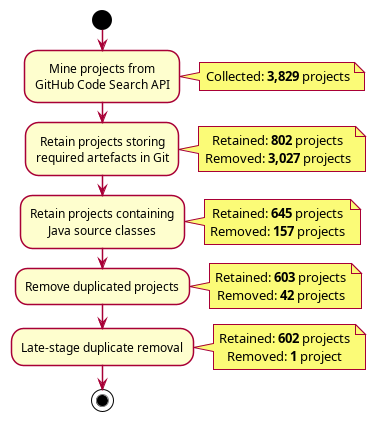
\includegraphics[width=200pt]{figures/data_funnel_diagram.png}
    \caption{Project mining and filtering stages.}
    \label{fig:dataFunnel}
\end{figure}

\subsection{Considered Alternatives}\label{sec:miningAlternatives}

Our method of mining repositories by using the GitHub code search API has the downside of being incomprehensive, meaning that it misses a portion of the projects available on GitHub for any of the following reasons:

\begin{itemize}
    \item the project does not use a build tool,
    \item the project uses a build tool that is not Maven or Gradle,
    \item the project is \textbf{only} found by search terms, which return over \num{1000} results, and the project is omitted due to not being indexed recently.
\end{itemize}

Although the portion of missed projects is low (no other Java build tool is anywhere near the popularity of Maven and Gradle \nobreakcite{stackOverflowSurvey}, and the more specific search terms should have caught all projects missed by the broader ones), it is a valid reason to mention alternative solutions we considered for mining Java repositories, and why we opted against using them.

\nobreaktextcite[p. 209]{allamanis2013mining} presented a curated corpus of \num{14807} open-source Java projects sourced from GitHub. As their work was published in 2013, it is outdated by 2026: a large part of the projects in the corpus has been deleted (as reported by \nobreaktextcite[p. 552]{goeminne2015towards} in 2015), new projects are missing, and the remaining projects could be using deprecated jOOQ APIs. Furthermore, their original corpus only contained ten projects using jOOQ \nobreakcite[Fig. 1]{goeminne2015towards}. 

We considered creating an up-to-date version of the corpus by repeating the work of Allamanis and Sutton, processing GitHub's event stream, provided by GH Archive \nobreakcite{ghArchive2026homepage}. However, the dataset has grown rapidly since 2013, and combined with the suboptimal structure of the GH Archive dataset \nobreakcite{ghArchiveLinkedIn}, it would have required us to commit an unreasonable amount of resources, given the preliminary nature of this research step. 

\nobreaktextcite[p. 58]{sharma2018smelly} employed RepoReaper \nobreakcite{DBLP:journals/ese/MunaiahKCN17} to select open-source repositories for their study, finding \num{2568} high-quality projects in various programming languages, which contained SQL statements. However, RepoReaper used GHTorrent \nobreakcite{DBLP:conf/msr/Gousios13} to obtain metadata about GitHub repositories \nobreakcite[p. 3223]{DBLP:journals/ese/MunaiahKCN17}, and GHTorrent has not been updated since early 2021 \nobreakcite{ghTorrentReddit}. Therefore, any set of projects produced based on GHTorrent would suffer from similar issues as the original corpus from Allamanis and Sutton.

Consequently, we found that our approach using the GitHub code search API is the best option available to us without committing unreasonable effort or resources.

\section{Establishment of Ground Truth}\label{sec:groundTruth}

To evaluate the detection performance of the prompting strategies and our later developed tool, we required a source of ground truth. As SQL antipatterns in jOOQ represent an unexplored area, to the best of our knowledge, no publicly available datasets of SQL antipatterns in jOOQ currently exist. Furthermore, the scientific literature provides no examples of how SQL antipatterns may occur in jOOQ, and such examples are also scarce elsewhere. For example, a remark in the jOOQ manual \nobreakcite{jooq2025select} shows that the “Implicit Columns” antipattern \nobreakcite[Ch. 19]{karwin2023sql} can occur in jOOQ in unexpected ways. Therefore, examples of antipatterns in plain SQL alone are insufficient for detecting SQL antipatterns in jOOQ.

To establish the ground truth, we manually annotated a subset of the projects gathered in Section~\ref{sec:mining}.

\subsection{Sample Generation}\label{sec:sampleGeneration}

As the projects are of varying size, we wanted the subset to be representative of the complete set of projects regarding size distribution, avoiding bias towards small or large projects. Figure~\ref{fig:distribution} displays the distribution of the number of relevant database access files per project across our dataset of \num{603} projects (still including the duplicated project that was filtered out at a later stage). We consider a Java source file to be a relevant database access file if both of the following conditions are met:

\begin{itemize}
  \item it is a jOOQ-generated file or contains references to jOOQ or a generated file,
  \item it is not considered “irrelevant” by a manually compiled path list.
\end{itemize}

 The path list consisted of jOOQ-generated files that were not useful for antipattern detection (e.g., records and POJOs), and files generated based on database entities not part of the project, such as system schemas of databases and tables managed by database extensions.

\begin{figure}[h]
    \centering
    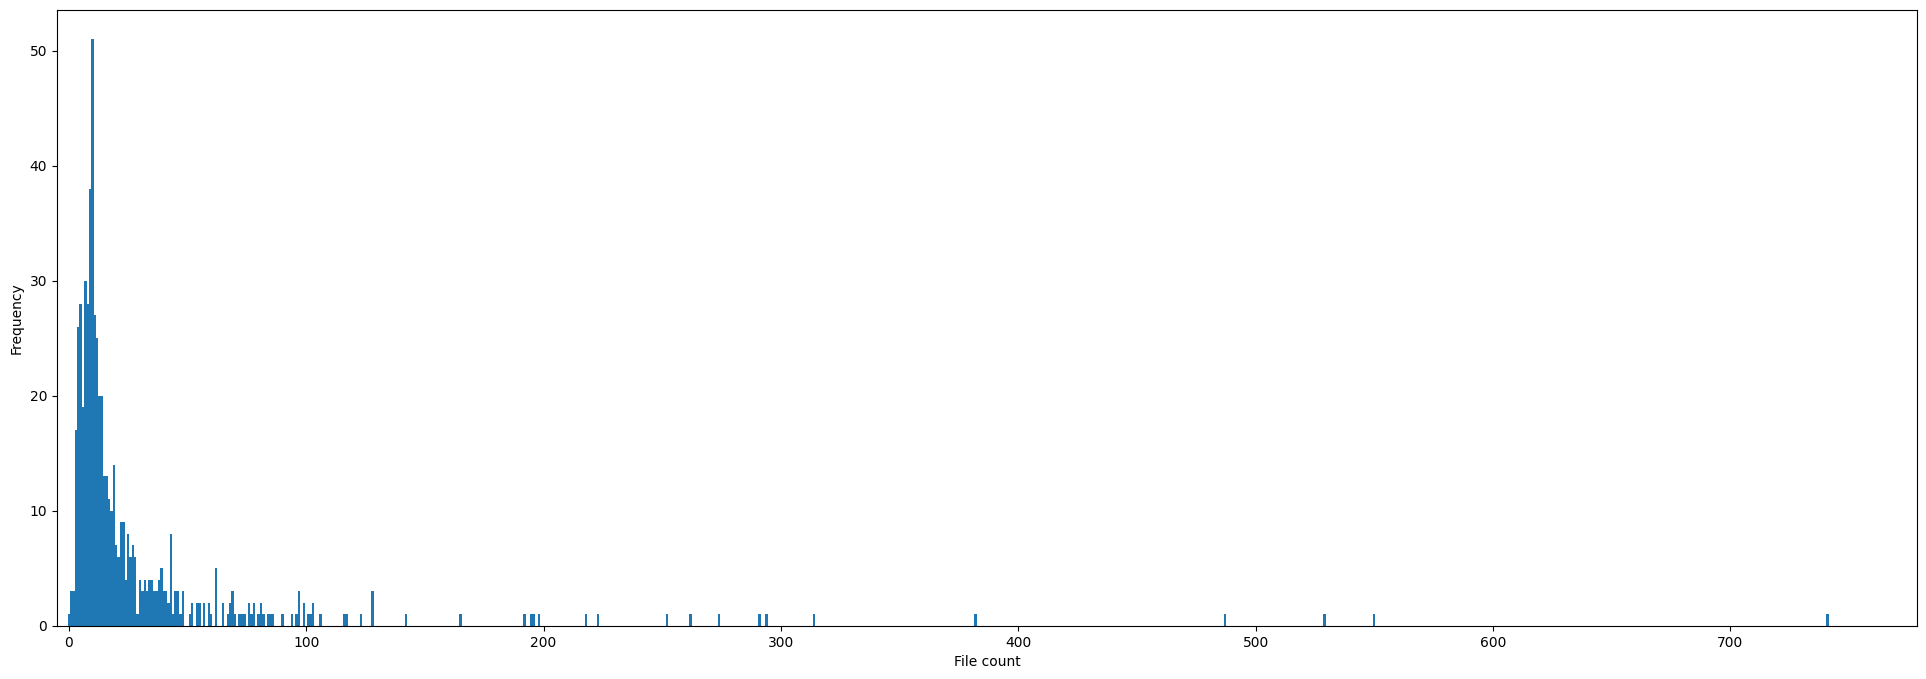
\includegraphics[width=\textwidth]{figures/distribution_of_files.png}
    \caption{Distribution of relevant database access files per project.}
    \label{fig:distribution}
\end{figure}

It should be noted that at this stage of the study, the list of “irrelevant” files was inconclusive and had some omissions, which we only discovered later. In Figure~\ref{fig:distributionCorrected}, we show the file distribution of 602 projects, omitting the later-discovered duplicated project, as well as using the final file list from a later stage of the study. It can be seen that, while the graph shifts slightly, the overall distribution remains similar.

\begin{figure}[h]
    \centering
    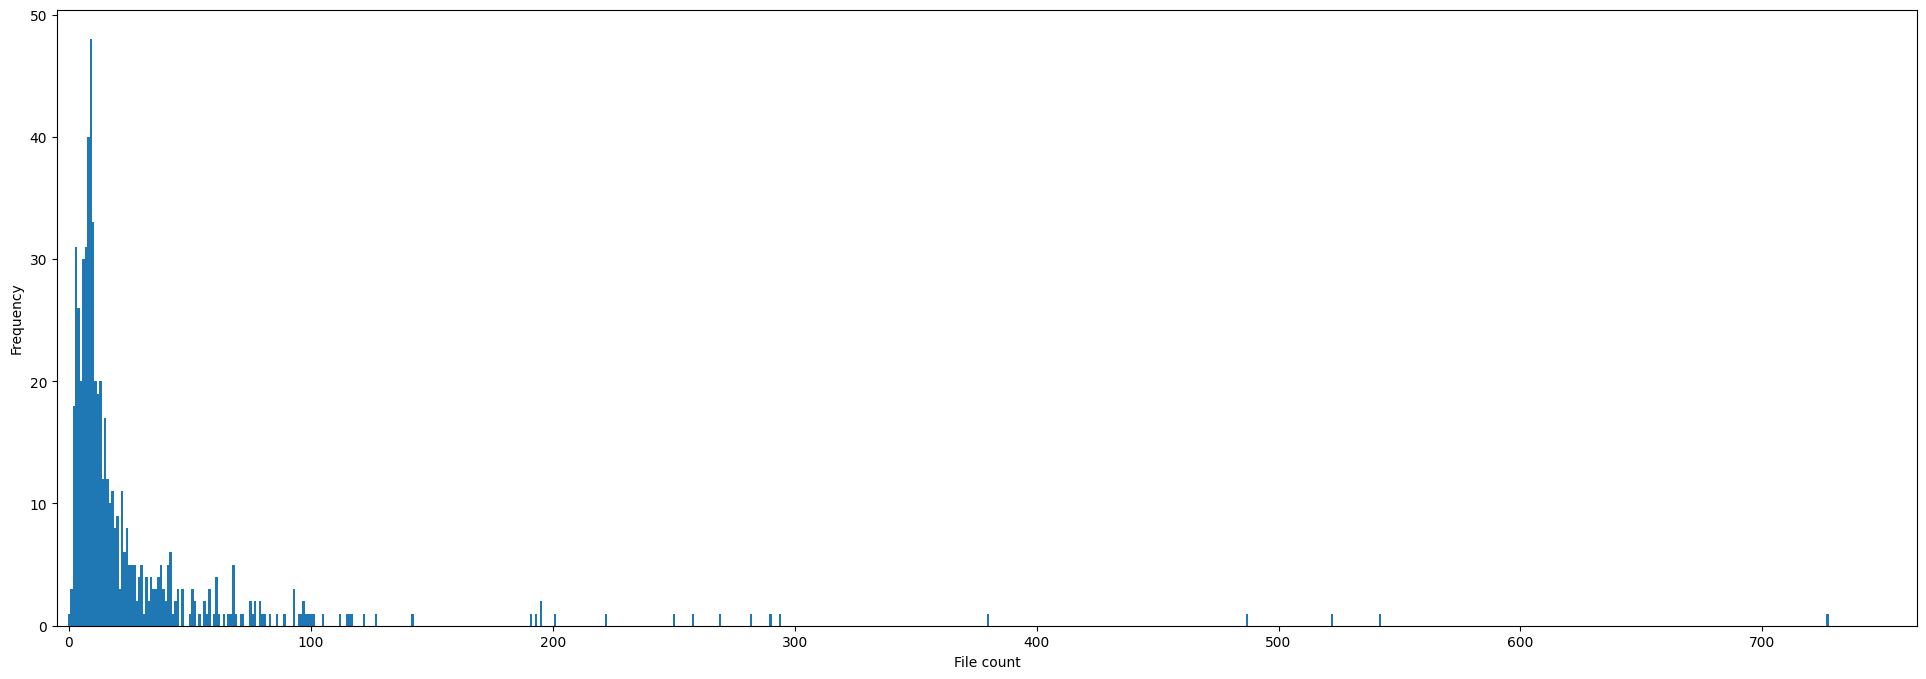
\includegraphics[width=\textwidth]{figures/distribution_of_files_corrected.png}
    \caption{Distribution of relevant database access files per project (corrected).}
    \label{fig:distributionCorrected}
\end{figure}

As illustrated in the figures, the project distribution is positively skewed, with most projects clustered near zero (the “head”) and a small number of substantially larger projects forming the “long tail”. To ensure that small, medium, and large projects are adequately represented, we employed a stratified random sampling approach, selecting an equal percentage of projects from each group. Our initial plan was to select \qty{5}{\percent} of the projects, but we later increased it to \textbf{\qty{10}{\percent}} due to an insufficient number of antipattern samples.

We divided the projects into size groups using the Head-Tail Breaks method. Given the set of projects as \(S\) and an individual project \(x\), we calculated the two breakpoints, \(\mu_1\) and \(\mu_2\), which represent the upper file limits for small and medium projects:
\begin{equation}
\mu_1 = \frac{1}{|S|} \sum_{x \in S} x
\end{equation}
\begin{equation}
S_{head} = \{ x \in S \mid x > \mu_1 \}
\end{equation}
\begin{equation}
\mu_2 = \frac{1}{|S_{head}|} \sum_{x \in S_{head}} x
\end{equation}

Based on these breakpoints, we classified the projects as:
\begin{equation}
\text{Class} = \begin{cases} 
      \text{Small} & x \le \mu_1 \\
      \text{Medium} & \mu_1 < x \le \mu_2 \\
      \text{Large} & x > \mu_2 
   \end{cases}
\end{equation}

We found the breakpoints to be \textbf{\num{31}} and \textbf{\num{94}}. Using these breakpoints, we classified \num{467} projects as small, \num{100} projects as medium, and \num{36} projects as large. Using the distribution from Figure~\ref{fig:distributionCorrected}, the numbers would have been slightly altered: the breakpoints would have been \num{29} and \num{91}, and the class sizes would have been \num{468}, \num{98}, and \num{36}.

Using the former classifications, we sampled \qty{10}{\percent} of projects from each size class, resulting in \num{47} small, ten medium, and four large projects. In total, the sample of projects selected for annotation contained \textbf{61} projects. We used the fixed seed \num{123456} for the pseudo-random number generator used for sampling, which ensures that the sampling process is consistent and reproducible.

\subsection{Antipattern Selection}\label{sec:antipatternSelection}

We limited the annotated antipatterns to the ones defined by \nobreaktextcite{karwin2023sql}. Although we attempted to maximise the number of antipatterns included in our analysis and to interpret them as closely as possible to Karwin’s definitions, we made several notable exclusions and interpretational deviations.

We excluded the “Index Shotgun” antipattern from our analysis. \nobreaktextcite[pp. 147--152]{karwin2023sql} recommends using the MENTOR (Measure, Explain, Nominate, Test, Optimize, and Rebuild) framework to choose optimal indexes. The framework involves measuring the runtime performance of SQL queries—a step that cannot be replaced by static analysis. Although other practitioners, such as \nobreaktextcite[pp. vi-vii]{Winand2012}, recommend creating optimal indexes during the development process, which could be aided by static analysis, choosing optimal indexes for a table can be a complex process with many trade-offs and deserves more dedicated research to be addressed appropriately.

We restricted our definition of the “Fear of the Unknown” antipattern to only include occurrences that are caused by flawed database design, as well as query conditions, which do not contain values passed in from Java code. As the type system of Java is not null-safe, Java code can contain many potential nullability errors, but detecting them would have caused a large additional annotation burden. Furthermore, specialised tools (e.g., NullAway \nobreakcite{DBLP:conf/sigsoft/BanerjeeCS19}) exist for detecting nullability errors in Java more efficiently and accurately.

\nobreaktextcite[p. 151]{nagy2017static} excluded the “Spaghetti Query” antipattern from their analysis, arguing that there is no objective definition to determine whether a query is a spaghetti query or not. They considered metrics, such as the length of a query in lines or characters, and counts of joins and subqueries, but found them too subjective.

Such metrics also do not tell the full picture, since one large query can often outperform multiple small queries due to optimisations in the database engine, and two queries with a similar length, involving the same number of tables, can differ vastly in their readability and performance. For example, \nobreaktextcite{Dombrovskaya2024} describe several techniques for factoring large queries to improve their performance, readability, or reusability. Furthermore, the use of jOOQ DSL makes it possible to factor the source code of queries using object-oriented principles, further aiding with readability and reusability. For these reasons, we excluded the “Spaghetti Query” antipattern from our analysis.

We extended our definition of “Implicit Columns” to also include other types of blind projections, which select every column from a table, such as API methods, which fetch generated records from the database \nobreakcite{jooq2025select}. Such blind projections are considered a bad practice according to the jOOQ documentation, having similar negative effects to the cases described by Karwin \nobreakcite{jooq2025select}.

We also excluded “Pseudokey Neat-Freak” and “Diplomatic Immunity” from our analysis, since they are rooted in organisational culture and cannot be detected from source code. Additionally, the use of jOOQ DSL largely mitigates the “Diplomatic Immunity” antipattern because SQL statements become first-class citizens of Java code.

Finally, we excluded the “See No Evil” antipattern due to difficulties in detecting it without performing runtime analysis. Unlike the Python examples provided by Karwin \nobreakcite[p. 270]{karwin2023sql}, Java projects using modern application frameworks do not usually perform fine-grained database exception handling for each database-related statement, but apply a retry mechanism at a transaction boundary, or use global exception handlers (e.g., in Spring \nobreakcite{spring2026exceptionHandler} and Micronaut \nobreakcite{micronaut2026exceptionHandler}), which could be implicitly installed by the framework. This makes accurate detection of the antipattern difficult for both human annotators and static analysis tools.

In total, we selected 19 antipatterns for annotation, including 8 logical design antipatterns, 3 physical design antipatterns, 5 query antipatterns, and 3 application development antipatterns. The list of included antipatterns by category is provided in Appendix~\ref{chapter:appendix-annotated-antipatterns}.

\subsection{Annotation Process}

Based on prior experience with jOOQ and SQL antipatterns, we manually assigned labels to antipattern occurrences found in the 61 sampled projects by carefully manually reviewing their source code. We tracked the labels in a LibreOffice spreadsheet, which we later converted into a comma-separated values (CSV) file. For each antipattern occurrence, we marked down the following information:
\begin{itemize}
    \item the type of antipattern,
    \item the project containing it,
    \item the path of the file containing it, relative to the root directory of the project,
    \item the start and end of the line span of the occurrence,
    \item a brief remark about the occurrence.
\end{itemize}

Due to the wide variety of Java versions, build tools, and local deployment methods used in the projects, along with occasional unavailable dependencies, we did not perform any runtime analysis on the projects.

As we studied a novel intersection between jOOQ and SQL antipatterns, not enough annotators sufficiently qualified in both domains were available to achieve a multi-annotator setup. Consequently, we employed a single-annotator setup, utilising the following means to maximise internal consistency.

\subsubsection*{Iterative Guideline Development}

During the annotation process, we created a codebook for the annotation process in the form of flowcharts available in Appendix~\ref{chapter:appendix-annotation-process-diagrams}.

During the annotation process, we followed the flowcharts for each antipattern, annotating their occurrences based on the visualised decision trees. When we spotted a variation of an antipattern or a non-antipattern edge case not yet covered by the corresponding decision tree, we adjusted the tree and re-reviewed previously, potentially incorrectly annotated files for consistency. This ensured that annotation decisions were made according to a consistent set of rules, rather than gut feeling.

\subsubsection*{Intra-Annotator Agreement}

After a 30-day washout period, we re-annotated a subset of the previously reviewed files to verify the stability of the annotation logic over time. We sampled \qty{10}{\percent} of the files containing at least one antipattern occurrence, and added an equivalent number of random files without antipattern occurrences to them. In total, we re-annotated \num{128} files using the same annotation guidelines. We used the fixed seed \num{123456} for the pseudo-random number generator used for sampling, which ensures that the sampling process is consistent and reproducible.

To measure the agreement between the two sets of annotations, we employed Cohen's Kappa ($\kappa$). However, traditional Kappa is designed for nominal classification and does not account for the spatial displacement inherent in a multi-occurrence localisation task. Consequently, we adapted the metric to determine whether the two sets of annotations contain the same antipattern occurrences based on an exact spatial match.

We define a line span \(S\) as the set of line indices within an inclusive range in a source code file.
\begin{equation}
S = \{i \in \mathbb{N} \mid start \le i \le end\}
\end{equation}

Given two annotators \(A\) and \(B\), and their annotated line spans \(S_A\) and \(S_B\), we consider the two line spans to match only if they cover the identical range of lines:
\begin{equation}
S_A = S_B
\end{equation}

After aligning the spans using this exact-matching gate, we constructed a \num{16} × \num{16} confusion matrix whose rows and columns represented the \num{15} distinct antipatterns annotated across the \num{128} files, together with the absence of an antipattern. The complete matrix is provided in Appendix~\ref{chapter:appendix-annotation-confusion-matrix}.

Given a set of \(k\) antipattern categories plus a “Background” category (\(k+1\) total classes), let \(n_{ij}\) denote the number of occurrences where Annotator A assigned class \(i\) and Annotator B assigned class \(j\). The total number of unique candidate occurrences is \(N = \sum_{i=1}^{k+1} \sum_{j=1}^{k+1} n_{ij}\).

The observed relative agreement (\(p_o\)) is defined as the proportion of occurrences where both annotators assigned the identical label to a spatially matching span:
\begin{equation}
p_o = \frac{1}{N} \sum_{i=1}^{k+1} n_{ii}
\end{equation}

The probability of random agreement (\(p_e\)) is calculated based on the marginal totals of the confusion matrix. Let \(n_{i \cdot}\) be the total number of times Annotator A used label \(i\), and \(n_{\cdot i}\) be the total number of times Annotator B used label \(i\). The expected agreement is defined as:
\begin{equation}
p_e = \frac{1}{N^2} \sum_{i=1}^{k+1} n_{i \cdot} n_{\cdot i}
\end{equation}

Where the marginal totals are derived as:
\begin{equation}
n_{i \cdot} = \sum_{j=1}^{k+1} n_{ij}, \quad n_{\cdot i} = \sum_{j=1}^{k+1} n_{ji}
\end{equation}

Finally, Cohen’s Kappa (\(\kappa\)) is computed to normalise the observed agreement against the possibility of chance:
\begin{equation}
\kappa = \frac{p_o - p_e}{1 - p_e}
\end{equation}

We found the Cohen's Kappa to be \textbf{\num{0.834}}. According to the standard scale by \nobreaktextcite{Landis77}, this represents an almost perfect agreement between the sets of annotations, demonstrating that the resulting dataset is internally consistent. Despite this, we acknowledge that the lack of an inter-annotator agreement check ultimately leaves the dataset vulnerable to the systematic blind spots of a single annotator.

\subsubsection*{Results}

In total, we annotated \textbf{\num{1562}} occurrences of 19 distinct SQL antipatterns within the \num{61} sampled projects. At least one occurrence of each antipattern was found in the sample, and every project in the sample contained at least one SQL antipattern occurrence. The most common antipatterns were “Implicit Columns”, which we found \num{795} occurrences of in 59 projects, and “ID Required” with \num{259} occurrences in \num{49} projects. In Table~\ref{tab:prevalenceInSample}, we show the prevalence of each SQL antipattern in the sampled projects.

\begin{longtable}[hp]{|p{3.5cm}|S[table-format=3, table-column-width=2cm]|S[table-format=2, table-column-width=2.5cm]|S[table-format=2.2, table-column-width=2.5cm]|S[table-format=2.2, table-column-width=3cm]|}
	\caption{Prevalence of SQL antipatterns in sampled projects.}
	\label{tab:prevalenceInSample}\\ \hline
	{\thead[l]{Antipattern}} & {\thead{Occurrence\\Count}} & {\thead{Containing\\Project Count}} & {\thead{Occurrences\\per Project}} & {\thead{Occurrences per\\Containing Project}}  \\
	\hline
	\endfirsthead
	\multicolumn{5}{l}
	{\tablename\ \thetable\ -- \textit{Continues...}} \\
	\hline
	{\thead[l]{Antipattern}} & {\thead{Occurrence\\Count}} & {\thead{Containing\\Project Count}} & {\thead{Occurrences\\per Project}} & {\thead{Occurrences per\\Containing Project}}  \\
	\hline
	\endhead
	\hline \multicolumn{5}{l}{\textit{Continues...}} \\
	\endfoot
	\hline
	\endlastfoot
    Implicit Columns & 795 & 59 & 13.03 & 13.47 \\ \hline
    ID Required & 259 & 49 & 4.25 & 5.29 \\ \hline
    Keyless Entry & 122 & 11 & 2.00 & 11.09 \\ \hline
    Fear of the Unknown & 95 & 19 & 1.56 & 5.00 \\ \hline
    31 Flavors & 71 & 11 & 1.16 & 6.45 \\ \hline
    \makecell[l]{Poor Man's\\Search Engine} & 55 & 12 & 0.90 & 4.58 \\ \hline
    \makecell[l]{Polymorphic\\Associations} & 40 & 1 & 0.66 & 40.00 \\ \hline
    Rounding Errors & 39 & 7 & 0.64 & 5.57 \\ \hline
    Ambiguous Groups & 24 & 2 & 0.39 & 12.00 \\ \hline
    Readable Passwords & 14 & 9 & 0.23 & 1.56 \\ \hline
    Phantom Files & 10 & 8 & 0.16 & 1.25 \\ \hline
    Naive Trees & 10 & 4 & 0.16 & 2.50 \\ \hline
    \makecell[l]{Standard Operating\\Procedures} & 8 & 1 & 0.13 & 8.00 \\ \hline
    Jaywalking & 6 & 2 & 0.10 & 3.00 \\ \hline
    Metadata Tribbles & 5 & 3 & 0.08 & 1.67 \\ \hline
    Entity-Attribute-Value & 3 & 3 & 0.05 & 1.00 \\ \hline
    SQL Injection & 3 & 1 & 0.05 & 3.00 \\ \hline
    Random Selection & 2 & 1 & 0.03 & 2.00 \\ \hline
    \makecell[l]{Multicolumn\\Attributes} & 1 & 1 & 0.02 & 1.00 \\
\end{longtable}

\subsection{Training-Validation-Test Split}\label{sec:dataSplit}

We divided the set of annotated projects into the following three subsets:

\begin{itemize}
    \item \textbf{Training set:} Used to continuously evaluate prompts during their development in Section~\ref{sec:prompts}. Also used as a source of examples for Few-Shot prompts.
    \item \textbf{Validation set:} Used to evaluate the detection performance of models and prompting strategies in Section~\ref{sec:experimentsQuantitative}.
    \item \textbf{Test set:} Used to evaluate the detection performance of the final tool in Section~\ref{sec:developmentQuantitative}.
\end{itemize}

To avoid developing our prompts and evaluating them on files obtained from the same projects, we assigned projects to subsets as wholes, rather than splitting their files between different subsets.

We fixed the seed of the pseudo-random number generator used for splitting to ensure that the splitting process was consistent and reproducible, but we were unable to use the previously used fixed seed \num{123456}, since the produced splits were heavily unbalanced.

To achieve an optimally balanced data split, we employed a seed search based on the Monte Carlo optimisation method. We iterated over seeds in the range of \num{0} to \num{1000000}, created a \num{34}/\num{33}/\num{33} training/validation/test split based on each seed, and calculated the sum of squared Coefficient of Variation (\(CV\)) for each split. We finally chose the split with the lowest sum of squared \(CV\).

Given an individual antipattern \(x\), a split \(i\) (assuming three splits), and the count of antipattern \(x\) occurrences in split \(i\) as \(C_{i,x}\), we define \(CV\) for an individual antipattern as:
\begin{equation}
\mu_x = \frac{1}{3} \sum_{i=1}^{3} C_{i,x}
\end{equation}
\begin{equation}
\sigma_x = \sqrt{\frac{1}{3} \sum_{i=1}^{3} (C_{i,x} - \mu_x)^2}
\end{equation}
\begin{equation}
CV_x = \frac{\sigma_x}{\mu_x}
\end{equation}

Then, given the set of antipatterns \(M\), we performed the optimisation:
\begin{equation}
\Phi = \sum_{j=1}^{M} \left( \frac{\sigma(x_j)}{\mu(x_j)} \right)^2
\end{equation}

To ensure statistical validity, we applied filtering criteria before performing the search. We excluded all antipatterns that appeared in fewer than three projects or had fewer than \num{25} total occurrences. Consequently, 12 of the initially annotated 19 antipatterns were excluded due to insufficient data. All subsequent experiments, tool development, and large-scale analyses in this thesis focus exclusively on the remaining seven qualifying antipatterns (listed in Table~\ref{tab:trainingTestValidationSplit}).

During this step, we also reconsidered the sample size for Section~\ref{sec:sampleGeneration}, first increasing it from \qty{5}{\percent} to \qty{7}{\percent}, and then to \qty{10}{\percent} of all projects, providing the search with a larger number of distinct project combinations and achieving a more balanced split.

The Monte Carlo optimisation-based search determined that the best possible split in this range was produced using the seed \num{767573}, which achieved a balance score of \num{0.52}. The distribution of antipattern occurrences between the datasets can be seen in Table~\ref{tab:trainingTestValidationSplit}.

\begin{longtable}[hp]{|p{4cm}|S[table-format=3, table-column-width=2cm]|S[table-format=3, table-column-width=2cm]|S[table-format=3, table-column-width=2cm]|S[table-format=3, table-column-width=2cm]|}
	\caption{Split of SQL antipattern occurrences between datasets.}
	\label{tab:trainingTestValidationSplit} \\ \hline
	{\thead[l]{Antipattern}} & {\thead{Total}} & {\thead{Training}} & {\thead{Validation}} & {\thead{Test}} \\
	\hline
	\endfirsthead
	\multicolumn{5}{l}
	{\tablename\ \thetable\ -- \textit{Continues...}} \\
	\hline
	{\thead[l]{Antipattern}} & {\thead{Total}} & {\thead{Training}} & {\thead{Validation}} & {\thead{Test}} \\
	\hline
	\endhead
	\hline \multicolumn{5}{l}{\textit{Continues...}} \\
	\endfoot
	\hline
	\endlastfoot
    Implicit Columns          & 795 & 175 & 350 & 270 \\ \hline
    ID Required               & 259 & 55  & 99  & 105 \\ \hline
    Keyless Entry             & 122 & 30  & 56  & 36  \\ \hline
    Fear of the Unknown       & 95  & 23  & 36  & 36  \\ \hline
    31 Flavors                & 71  & 17  & 15  & 39  \\ \hline
    Poor Man's Search Engine  & 55  & 19  & 15  & 21  \\ \hline
    Rounding Errors           & 39  & 13  & 10  & 16  \\
\end{longtable}

All produced datasets, along with their intended use cases later in the study, are visualised in Figure~\ref{fig:dataSets}.

\begin{figure}[h]
    \centering
    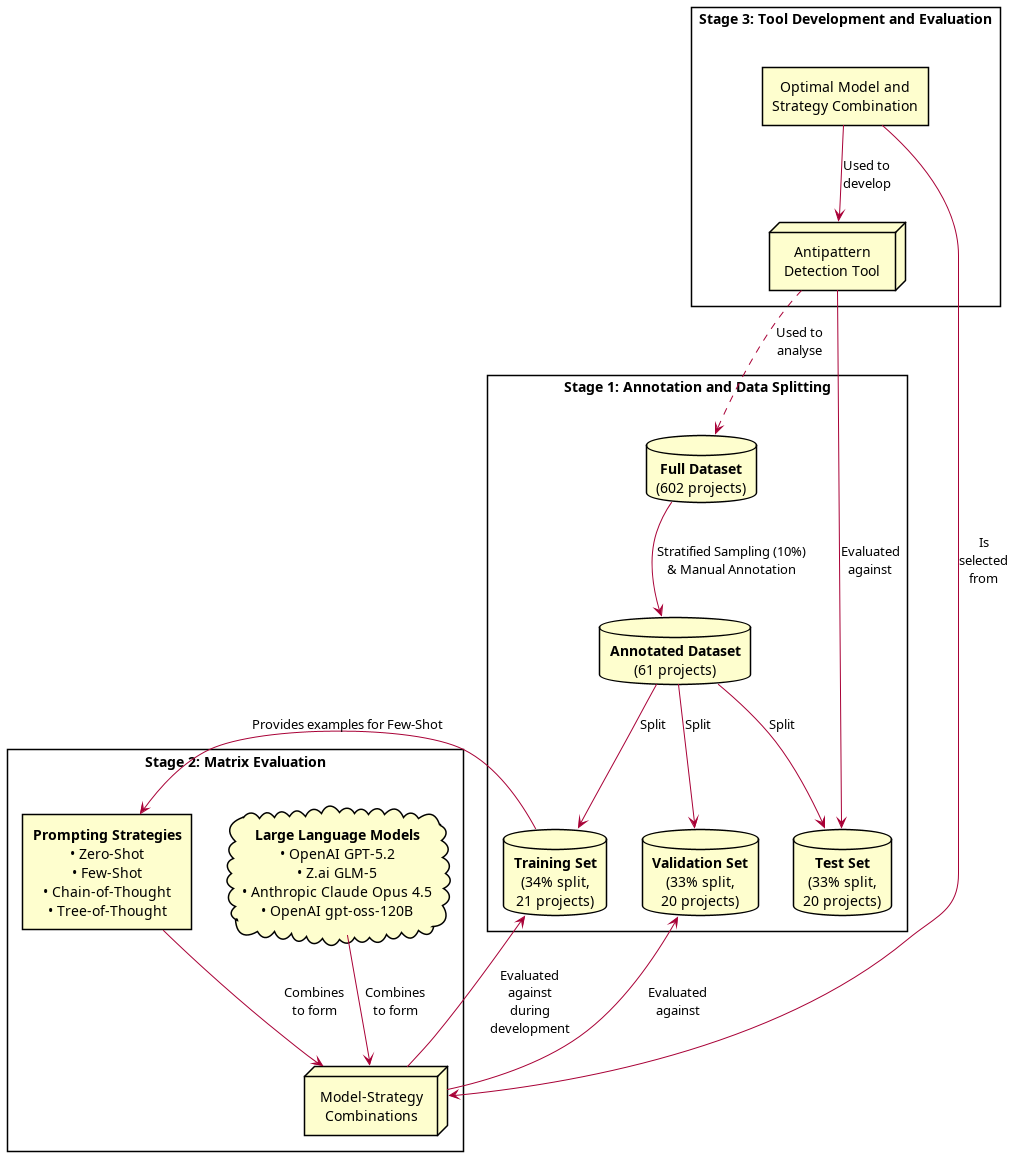
\includegraphics[width=\textwidth]{figures/data_sets_diagram.png}
    \caption{All created datasets with their intended uses.}
    \label{fig:dataSets}
\end{figure}


\chapter{Evaluation of Prompting Strategies}\label{chapter:promptingStrategies}
This chapter details the empirical evaluation of various prompting strategies for detecting SQL antipatterns in jOOQ. To assess the versatility and reliability of these strategies under different conditions, we benchmarked them across multiple contemporary LLMs, analysing both quantitative performance metrics and qualitative outputs.

\section{Selecting Models}\label{sec:models}

To assess the prompting strategies under varying conditions, we evaluated them against multiple models. We chose the language models based on criteria selected to aid us in the development and analysis process, while keeping the selection of models diverse. In particular, we searched for the following characteristics in the models:

\begin{itemize}
    \item \textbf{Architectural diversity:} We aimed to include models with a diverse set of characteristics, such as different model sizes, reasoning vs non-reasoning models, and open vs closed-weight models.
    \item \textbf{Performance:} For a given architecture, the model should demonstrate near-state-of-the-art (SotA) performance on public benchmarks \nobreakcite{artificialAnalysis}.
    \item \textbf{Repeatability:} The weights of the model should be stable, allowing the evaluation and analysis to be repeated in the future. Ideally, the model should have open weights. Alternatively, the model provider should provide point-in-time snapshots of the model.
    \item \textbf{Structured outputs:} The model should reliably support structured outputs, providing responses that reliably adhere to expected JSON Schema. This was desired to avoid the complexity of parsing non-structured outputs and handling of malformed responses. Structured output also increases determinism in responses by constraining decoding to outputs that satisfy the schema \nobreakcite{structuredOutputs}.
\end{itemize}

Based on this set of criteria, we settled on the following four models for our analysis:

\begin{itemize}
    \item \textbf{OpenAI GPT-5.2 \nobreakcite{gpt52} (reasoning):} Near-SotA proprietary weights model. The best-performing model offering point-in-time snapshots.
    \item \textbf{Z.ai GLM-5 \nobreakcite{DBLP:journals/corr/abs-2602-15763} (reasoning):} SotA open-weights model.
    \item \textbf{Anthropic Claude Opus 4.5 \nobreakcite{opus45Card} (non-reasoning):} Near-SotA in models, which allow reasoning to be disabled. Superseded by Opus 4.6, which did not offer point-in-time snapshots at the time.
    \item \textbf{OpenAI gpt-oss-120B \nobreakcite{DBLP:journals/corr/abs-2508-10925} (reasoning):} Open-weights, SotA in models classified as medium language models (up to \num{150}B parameters).
\end{itemize}

Initially, we also planned to include Z.ai GLM-4.7-Flash \nobreakcite{DBLP:journals/corr/abs-2508-06471}, which was the best-performing small language model (up to \num{40}B parameters) at the time, but we were required to omit it due to vast stability issues with all providers offering the model.

We most notably omitted Google Gemini 3.1 Pro Preview \nobreakcite{gemini31ProPreview} and Anthropic Claude Opus 4.6 \nobreakcite{opus46Card}, which outperformed all the selected models, but due to their recent releases, did not have point-in-time snapshots available.

We were also not able to include any purely non-reasoning models in the comparison: such models have become increasingly rare, and the most capable purely non-reasoning model at the time, Kwaipilot KAT-Coder-Pro V1 \nobreakcite{DBLP:journals/corr/abs-2510-18779}, did not offer point-in-time snapshots. However, many modern reasoning models allow that capability to be disabled; therefore, we substituted the model with Anthropic Claude Opus 4.5, with the reasoning capability disabled.

We found that all selected models supported structured outputs with adequate reliability. In our preliminary experiments, some older models (e.g., Kimi K2 Thinking \nobreakcite{DBLP:journals/corr/abs-2507-20534}) did not adhere to the provided JSON Schema, causing client-side validation to fail in numerous cases, but such issues were much less common in the selected models. The complete set of models considered for the analysis, along with their inclusion and omission reasons, is available in Appendix~\ref{chapter:appendix-model-selection}.

\section{Designing Prompts}\label{sec:prompts}

We designed prompts based on the four prompting strategies listed in Section~\ref{sec:promptEngineering}. We limited our experiments to prompting techniques that could be fully executed in the span of one prompt and one response to manage the scope of the thesis.

We iteratively developed and fine-tuned prompts for each technique, comparing the results against the training set produced in Section~\ref{sec:dataSplit}. We tested each iteration of our prompts against all tested models until all models reached near-optimal performance. To simplify the experimental setup and the interpretation of results, we only developed universal, model-agnostic prompts, without fine-tuning them for individual models.

Due to the high cost of LLM inference, we developed heuristics to target only the antipatterns that are potentially present in a given file. Firstly, we ignored files that did not contain any database-related code using the filters first mentioned in Section~\ref{sec:sampleGeneration}. Secondly, for each prompting strategy, we developed two prompts: 

\begin{itemize}
    \item for detecting query antipatterns from non-generated source files,
    \item for detecting (mostly) design antipatterns from files generated by jOOQ.
\end{itemize}

In addition to the file being analysed, we provided the design antipattern detection prompts with additional context by supplying them with a jOOQ-generated class containing the definitions of all primary, unique, and foreign key constraints present in that database schema. This additional context is used in the detection of the “Keyless Entry” antipattern to verify if there is an appropriate primary or unique key present, which the missing foreign key could reference.

We also applied the following pre-processing steps to the input files:
\begin{itemize}
    \item To reduce the number of input tokens, and subsequently costs, we removed all leading and trailing whitespace from each line in the input files (including indentation).
    \item We noticed that the models consistently miscalculated the row spans of antipattern occurrences, if the analysed file contained two or more consecutive line breaks anywhere in the file before the antipattern occurrence. The models also often mislocated antipattern occurrences in large source files. To resolve these issues, we prefixed each line in the input file with the correct line number.
\end{itemize}

We designed our prompts to detect the seven qualifying antipatterns present in the training, validation, and tests sets created in Section~\ref{sec:dataSplit}. Designing them, we started with broad instructions, allowing models to use their judgement and reasoning to a wide extent. As we identified instances where the model misinterpreted certain antipatterns or detected them incorrectly, we moved towards more concrete and specific instructions to eliminate ambiguity and ensure the model consistently adhered to our intended criteria.

Ultimately, it was necessary to define all detected antipatterns explicitly and, in certain cases, to specify the exact method calls and coding patterns to look out for. When models were provided only with the names of antipatterns, they tended to construct their own definitions, which were at times inconsistent with those proposed by \nobreaktextcite{karwin2023sql}. We attribute this behaviour to the limited availability of literature on SQL antipatterns within the training data of LLMs, resulting in them “hallucinating” the definitions. 

Furthermore, for the “ID Required”, “31 Flavors”, “Poor Man's Search Engine”, and “Implicit Columns” antipatterns, it was necessary to provide explicit localisation rules to ensure consistent localisation behaviour.

For the Few-Shot Prompting technique, which required concrete examples, we acquired the examples from the training set produced in Section~\ref{sec:dataSplit} by default. For antipattern variants and edge cases, which we were unable to find representative examples for from the training set, we created the examples synthetically.

We ultimately settled on the instructions detailed in Figures~\ref{fig:ddlInstructions} and~\ref{fig:dmlDqlInstructions} for detecting antipatterns in generated and non-generated source files, respectively, consistent between all prompting strategies listed in Section~\ref{sec:promptEngineering}. The complete prompts for all prompting strategies, containing sample input files, are shown in Appendix~\ref{chapter:appendix-final-prompts}.

\bigskip % Add space before the figure
\begingroup % Start a local scope
\captionsetup{type=figure}
\phantomsection
\captionlistentry[figure]{Detection instructions used in DDL prompts.}\label{fig:ddlInstructions}
\begin{lstlisting}[
    frame=none, 
    basicstyle=\small, 
    breaklines=true, 
    breakatwhitespace=false, 
    breakindent=0pt
]
- ID Required: Never identify this issue in classes representing views, as views cannot contain primary keys. If the class represents a table, always detect the antipattern, if the name of the primary key is just "id" (case-insensitive). Also detect the issue if a synthetic primary key column exists, even though another unique constraint exists, which is suitable as a primary key (the constraint is on columns, which are virtually immutable by nature), and which does not complicate foreign keys referencing the table too much. Only include the lines of the primary key column definition in the line range, do not include comments or anything else.
- Keyless Entry: A column, which refers to another table, is missing its foreign key. Never identify this issue in classes representing views, as views cannot contain foreign keys. Only report this issue if the "Keys" class provided at the end contains a primary key that this is appropriate for this column to refer to.
- Rounding Errors: Storing fixed-precision values in floating-point type columns, such as FLOAT and REAL, rather than using fixed-precision types like DECIMAL and NUMERIC.
- 31 Flavors: Specifying allowed values in the column definition, i.e. with a CHECK constraint or an ENUM type, rather than using a lookup table. Only include the lines of the column definition in the line range, do not include comments or anything else. Do not report the issue if the CHECK constraint is used to check the value for emptiness or against a range of values (including greater/lesser than comparisons).
- Fear of the Unknown: A special default value, such as an empty string, is used to mark a missing value, rather than NULL, and the special value does not hold a semantic meaning. A column, which can never be NULL in practice (e.g. it has a default value), is marked as NULLABLE.

If the file does not contain any antipatterns, leave the list of occurrences empty.
\end{lstlisting}

\nopagebreak
\begin{minipage}{\linewidth}
    \captionof*{figure}{Figure \thefigure. Detection instructions used in DDL prompts.}
\end{minipage}
\par % Apply the paragraph settings *inside* the group
\endgroup % Revert to global normalsize and paragraph spacing

\bigskip % TODO: verify before submitting
\bigskip % these are here to make sure the caption for figure 8 is not on a new page alone

\begingroup % Start a local scope
\captionsetup{type=figure}
\phantomsection
\captionlistentry[figure]{Detection instructions used in DML/DQL prompts.}\label{fig:dmlDqlInstructions}
\begin{lstlisting}[
    frame=none, 
    basicstyle=\small, 
    breaklines=true, 
    breakatwhitespace=true, 
    breakindent=0pt
]
- Poor Man's Search Engine: Usage of LIKE, ILIKE or regular expressions to perform full-text search. Report the issue if it isn't obvious from the method input parameters, whether the patterns contain wildcards used for full-text search. Do not report the issue if LIKE, ILIKE or regex is used for prefix search. Only include the line(s) where the full-text search condition is created in the line range.
- Implicit Columns: A query fetching all columns from a database table. In addition to obvious violations, report cases where jOOQ fetches all columns of a table into records or generated DAOs (located in a package ending with `tables.daos`). Do not report this issue if it occurs within a `fetchCount` or `fetchExists` call. Only include the line(s) where the blind projection is selected in the line range, do not include the rest of the query.
- Fear of the Unknown: Query logic uses a NULLABLE column in a way that produces incorrect results with NULL. Do not report issues that arise from insufficient null-handling in Java code. Also do not report the issue if you're unsure if the column is NULLABLE.

Only identify problems in code, which interacts directly with the jOOQ DSL or generated DAOs (located in a package ending with `tables.daos`). Do not identify problems in code, which interacts with higher level abstractions. In case of multiple consecutive issues, report them separately, even if they are on consecutive lines. If the file does not contain any antipatterns, leave the list of occurrences empty.
\end{lstlisting}

\nopagebreak
\begin{minipage}{\linewidth}
    \captionof*{figure}{Figure \thefigure. Detection instructions used in DML/DQL prompts.}
\end{minipage}
\par % Apply the paragraph settings *inside* the group
\endgroup % Revert to global normalsize and paragraph spacing

\section{Quantitative Analysis}\label{sec:experimentsQuantitative}

Following the finalisation of the prompt design, we analysed each project in the validation set created in Section~\ref{sec:dataSplit} using all combinations of models and prompting strategies. We subsequently evaluated the resulting outputs against the ground truth.

We performed the analysis using the OpenAI Python SDK \nobreakcite{openAiPython2026GitHub}, accessing the models through OpenRouter \nobreakcite{openRouter2026homepage} as a unified gateway for different LLM providers, using the following parameters for LLMs:

\begin{itemize}
    \item \textbf{Temperature}: Used to control the randomness of the output, with higher values resulting in less deterministic results. Using a value of zero encourages the model to select the most likely token, reducing randomness and improving repeatability, making the output as deterministic as possible. We used the default value \num{1.0} for OpenAI gpt-oss-120B, since using near-zero values caused it to repeat tokens infinitely, and this issue did not resolve with any other parameter changes. We used the value \num{0.0} for all other models, except for OpenAI GPT-5.2, which did not support the parameter when being used as a reasoning model.
    \item \textbf{Effort}: Used to control how much internal reasoning the model performs before generating a response. Higher effort levels enable deeper, multi‑step analysis, generally improving reliability, while being slower, costlier, and less deterministic. We used the highest supported value for each reasoning model to leverage improved reliability, while compensating for decreased determinism with other techniques.
\end{itemize}

In Table~\ref{tab:modelParameters} we show the selected parameter combinations for each model used for analysis.

\begin{longtable}[hp]{|p{7.5cm}|S[table-format=1.1, table-column-width=3cm]|p{3cm}|}
	\caption{Model parameters used for analysis.}
	\label{tab:modelParameters}\\ \hline
	{\thead[l]{Model}} & {\thead{Temperature}} & {\thead{Effort}} \\
	\hline
	\endfirsthead
	\multicolumn{3}{l}
	{\tablename\ \thetable\ -- \textit{Continues...}} \\
	\hline
	{\thead[l]{Model}} & {\thead{Temperature}} & {\thead{Effort}} \\
	\hline
	\endhead
	\hline \multicolumn{3}{l}{\textit{Continues...}} \\
	\endfoot
	\hline
	\endlastfoot
    \sotaModel & {Unsupported} & xhigh \\ \hline
    \openModel & 0.0 & Unsupported \\ \hline
    \nonReasoningModel & 0.0 & none \\ \hline
    \mediumModel & 1.0 & high \\
\end{longtable}

While OpenRouter provides a convenient unified API, it acts as an abstraction layer where internal routing and caching semantics can vary. To maintain strict control over the experimental environment, we explicitly disabled OpenRouter's automatic model fallbacks. This ensured that requests were evaluated exclusively by the requested model or failed outright, triggering our local retry mechanism. We also considered OpenRouter's default request caching; however, because each analysed source file generated a strictly unique prompt and the evaluation was executed in a single pass, gateway-level caching could not artificially influence our results.

In essence, we were evaluating the performance of the models and prompts in performing a \textbf{multi-label} (there were multiple antipatterns that could be detected) \textbf{multi-occurrence} (each antipattern could occur multiple times within each file) \textbf{localisation} (in addition to classification, we aimed to detect the location of the antipattern occurrences) task. For this reason, we employed a combination of spatial overlap criteria and classification metrics for evaluation, using Intersection over Union (IoU) and F1-score.

The first step involved quantifying the localisation performance using IoU. We define a line span \(S\) as the set of line indices within an inclusive range in a source code file.
\begin{equation}
S = \{i \in \mathbb{N} \mid start \le i \le end\}
\end{equation}

For a predicted line span \(S_p\) and a ground truth line span \(S_g\), the IoU is defined as:
\begin{equation}
\text{IoU} = \frac{|S_p \cap S_g|}{|S_p \cup S_g|}
\end{equation}

This metric produces a value between \num{0} and \num{1}, where \num{1} represents an exact line-level match. In this methodology, the IoU serves as the qualification gate for all subsequent metrics. A prediction is classified as a true positive (TP) if its spatial overlap with the ground truth exceeds the threshold: \(\text{IoU} \geq 0.5\). If the IoU is below this threshold, the prediction is classified as a false positive (FP), while missed ground truth spans are considered false negatives (FN).

Using this qualification gate, we classify the predictions into TPs, FPs, and FNs, employing Non-Maximum Suppression (NMS): in cases of multi-occurrence where multiple predictions overlap a single ground truth span, only the prediction with the highest spatial overlap is assigned as a TP, while subsequent overlaps are penalised as FPs.

Based on the classifications, we calculated the precision (\(P\)) and recall (\(R\)) of the model at the selected threshold, defined as:
\begin{equation}
P = \frac{\text{TP}}{\text{TP} + \text{FP}}, \quad R = \frac{\text{TP}}{\text{TP} + \text{FN}}
\end{equation}

Precision measures the exactness of the model by calculating the ratio of correctly identified detections to the total number of detections, thereby indicating the extent to which the model avoids FPs. Recall measures the completeness of the model by calculating the ratio of correctly identified detections to the total number of antipattern occurrences in the ground truth, reflecting the model's ability to minimize FNs.

Using these values, we calculated the F1-score, which provides a balanced assessment of model performance at the selected threshold by calculating the harmonic mean of precision and recall, serving as a single unified metric that penalizes extreme values in either component:
\begin{equation}
F_1 = 2 \cdot \frac{P \cdot R}{P + R}
\end{equation}

We calculated \(P\), \(R\) and \(F_1\) for each antipattern separately, and as a weighted average of all antipatterns:
\begin{equation}
\bar{x}_w = \frac{\sum_{i=1}^{n} w_i x_i}{\sum_{i=1}^{n} w_i}
\end{equation}

This way, we were provided with an understanding of which models and prompts are the best in the detection of antipatterns in general, but we also had the opportunity to study the differences in further detail. Additionally, we recorded the cost and runtime of each analysis and the number of requests retried due to incorrectly formatted (e.g., empty or non-JSON) responses provided models.

We acquired the data about costs from the OpenRouter dashboard due to a subtlety in the OpenAI Python SDK's API for structured outputs: if the client-side validation for the output fails, the request, including its usage data, cannot be obtained from the client code, making accurate cost calculations impossible. We represent the cost in USD including VAT, and the runtime in seconds.

Based on the results of this analysis, we could provide answers to \textbf{RQ1} and \textbf{RQ2} in Sections~\ref{sec:resultsRQ1} and~\ref{sec:resultsRQ2}, and we could decide on the preferred prompting strategy for the development of an antipattern detection tool in Chapter~\ref{chapter:development}.

\section{Qualitative Analysis}

We manually inspected the results produced by each combination of model and prompting strategy. Where possible, we also inspected the reasoning data to identify behavioural patterns that could explain the frequent FPs and FNs in the results. We then compared our experimental findings with existing literature on prompting strategies and LLM behaviour.

We discuss the results of the qualitative analysis in Section~\ref{sec:llmCapabilities}.


\chapter{Development of Antipattern Detector}\label{chapter:development}
This chapter provides an overview of the developed command-line tool for detecting the seven targeted SQL antipatterns, which employs the most effective prompting strategy identified based on the analysis that was described in Section~\ref{sec:experimentsQuantitative}. We discuss the tool's architectural design, internal workflow, and configuration options, as well as the coding process used to implement it.

The tool was developed with the assistance of OpenAI Codex \nobreakcite{openAiCodex2026GitHub}, using the GPT-5.4 \nobreakcite{gpt54} model, in a semi-autonomous agentic coding process. The development process was organised around iterative implementation tasks. For each task, we specified the intended behaviour, constraints, and expected outcome, after which the coding agent inspected the existing codebase, proposed or implemented the necessary changes, and ran relevant checks where applicable. Human supervision was retained throughout the process: generated changes were reviewed, requirements were clarified when necessary, and architectural decisions, evaluation requirements, and final acceptance of the implementation remained under human control. In this way, Codex was used primarily as an implementation assistant, while the design goals and validation criteria were defined by us.

\section{Architecture}

We implemented the tool as a monolithic command-line interface (CLI) application. Compared to a graphical user interface (GUI) application, this approach offers greater versatility, allowing the tool to be run in non-interactive environments, such as continuous integration (CI) pipelines and batch evaluation scripts. Additionally, the CLI approach avoids coupling the core analysis logic to a particular user interface. This allows for developing alternative frontends in the future, such as a standalone desktop application or an IDE extension, without requiring substantial changes to the analysis pipeline.

The tool is built as a self-contained executable without local runtime dependencies (e.g., Python or Node.js), simplifying distribution and use in controlled evaluation environments. It features extensive configuration options (detailed in Section~\ref{sec:configurationOptions}), which can be provided as command-line options, environment variables, or in a configuration file. In case of duplicated options, command-line options take precedence over environment variables, which in turn take precedence over the configuration file.

A high-level diagram of the tool's architecture is shown in Figure~\ref{fig:toolComponents}.

\begin{figure}[h]
    \centering
    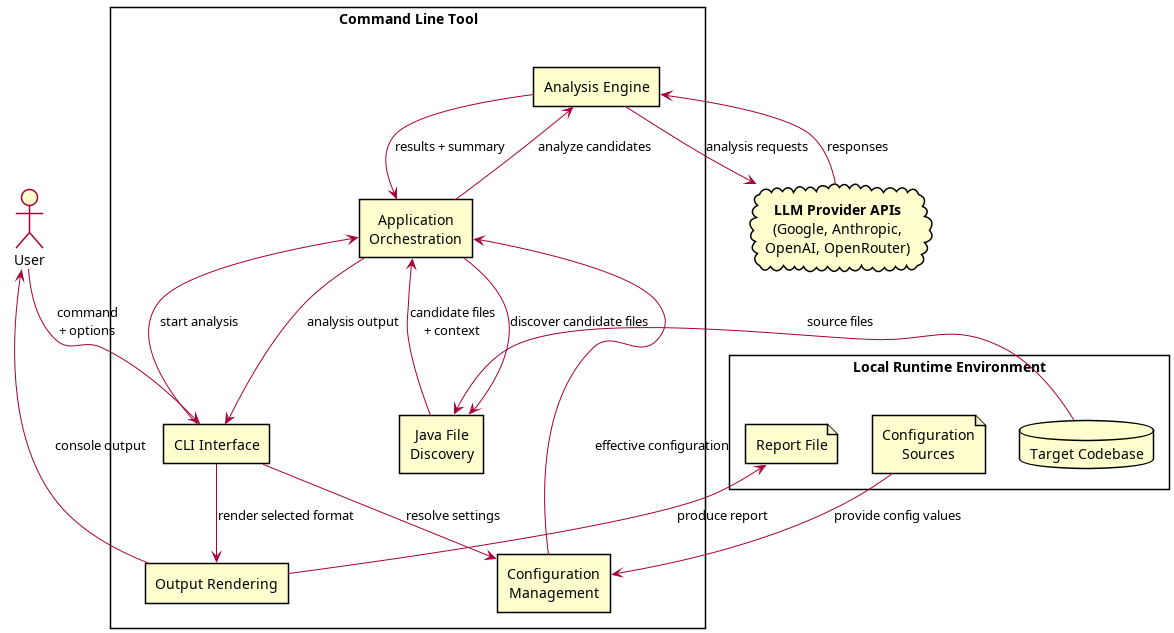
\includegraphics[width=\textwidth]{figures/component_diagram.png}
    \caption{Components of the SQL antipattern detection tool.}
    \label{fig:toolComponents}
\end{figure}

\section{Workflow}\label{sec:workflow}

Although the tool is implemented as a monolithic application, its internal architecture is organised as the staged pipeline shown in Figure~\ref{fig:toolWorkflow}. The main stages of the pipeline are the following:

\begin{itemize}
      \item \textbf{Input and configuration:} The tool receives command-line arguments, validates the input directory, and combines command-line options, environment variables, an optional configuration file, and built-in defaults into a single validated runtime configuration.
      \item \textbf{Model setup:} The selected model is resolved from an explicit provider-prefixed identifier. The provider prefix determines which LLM client is created and which API key is required.
      \item \textbf{Source-file discovery:} The selected project directory is recursively scanned for Java source files. The tool then applies jOOQ-oriented inclusion and exclusion heuristics to retain only files likely to contain relevant schema or query logic.
      \item \textbf{Candidate preparation:} Each retained Java file is converted into an analysis candidate containing its path, contents, analysis category, and optional contextual information. The analysis category determines whether the file is analysed as schema-definition code or query/application code. The tool also attaches the closest available key-definition context when such context is found.
      \item \textbf{Per-file analysis:} Candidate files are processed concurrently up to the configured concurrency limit. For each candidate, the source code is converted into a line-numbered representation and inserted into an LLM request. When the prompt-size budget requires it, the source context and any attached key-definition context are truncated while preserving useful context where possible.
      \item \textbf{Validation and failure handling:} If a request fails or returns data in an unexpected format, the tool retries it according to the configured retry count. If all attempts fail, the error is reported as a per-file result instead of aborting the whole run.
      \item \textbf{Aggregation and rendering:} After all candidates have been processed, the tool sorts the per-file results, computes a run-level summary, and renders the structured result as text, JSON, or CSV. The rendered output is then written either to standard output or to a configured output file.
\end{itemize}

\begin{figure}[H]
    \centering
    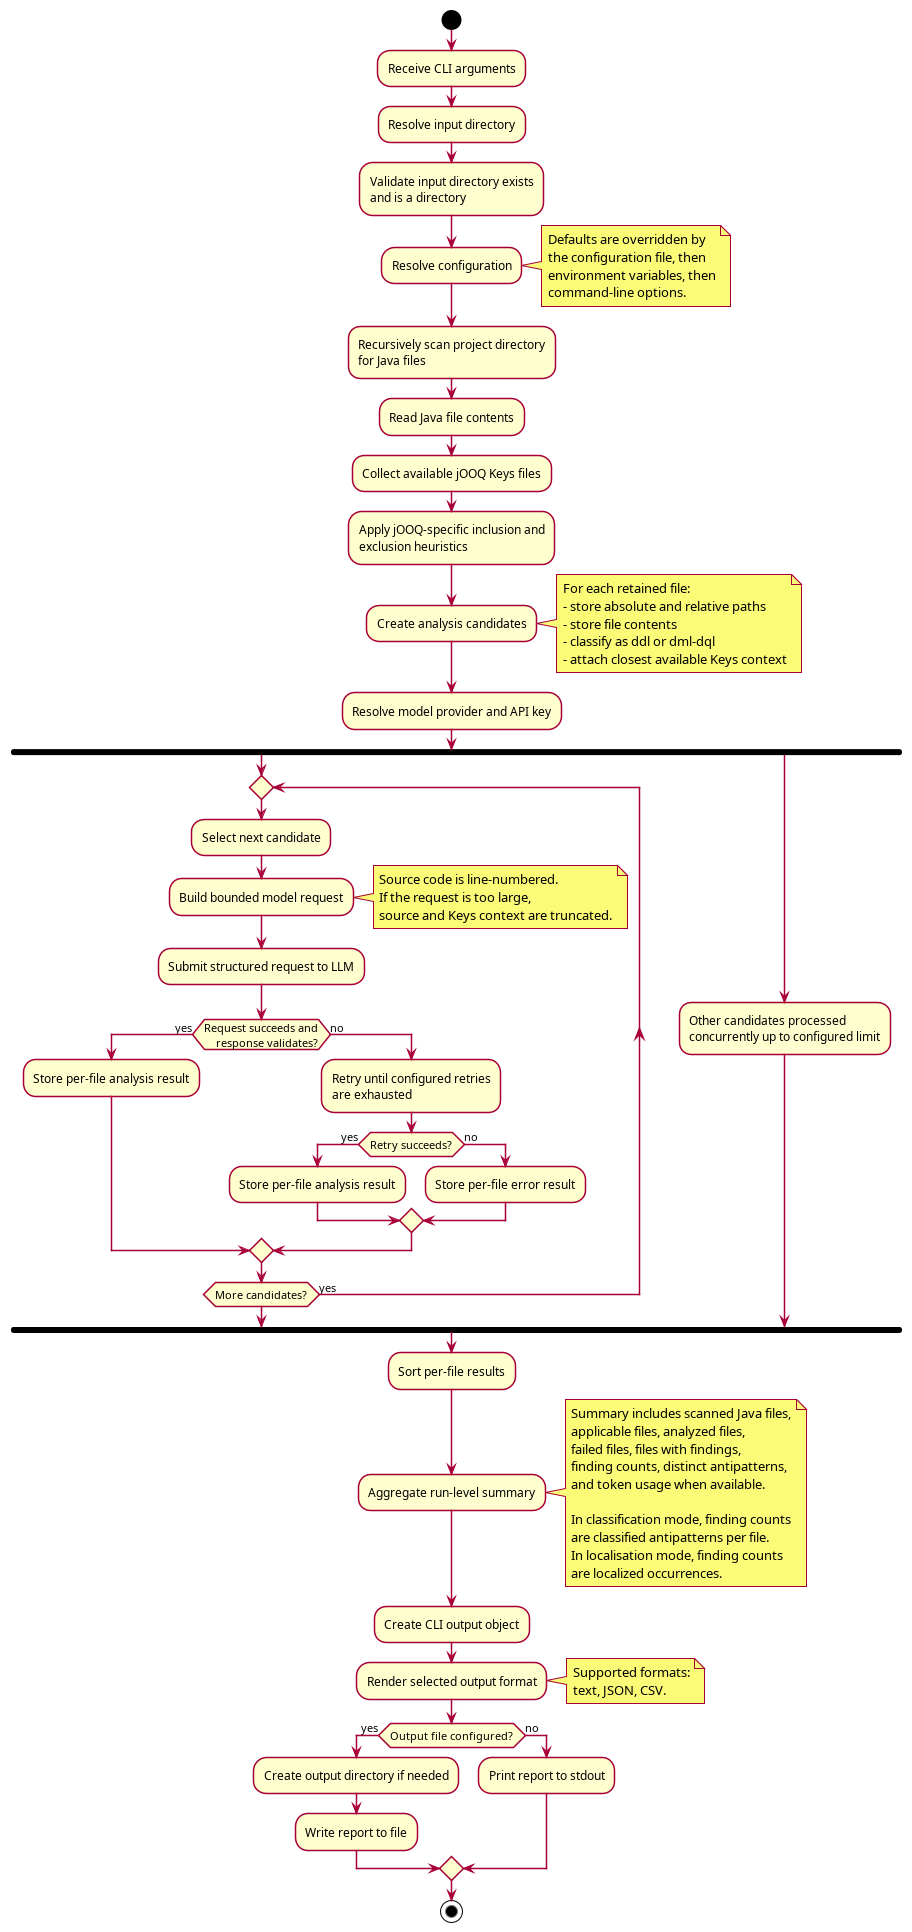
\includegraphics[width=320pt]{figures/tool_workflow.png}
    \caption{Workflow of the SQL antipattern detection tool.}
    \label{fig:toolWorkflow}
\end{figure}

\section{Result Representation}

The tool supports two analysis modes. In localisation mode, the output contains occurrence-level findings with source locations and explanations. In classification mode, the output contains only the distinct antipatterns detected in each file. The output of a run is a structured report consisting of run-level metadata, aggregate statistics, and per-file analysis results. The text rendering is intended for human inspection, while JSON and CSV outputs support automated processing, evaluation scripts, and integration with other tools.

Figure~\ref{fig:toolResults} shows a shortened text rendering of an analysis report in the localisation mode. The report begins with the selected model and analysed directory, followed by aggregate statistics. Individual findings are then grouped by file and include the detected antipattern, source location, relevant code fragment, and an explanation.

\bigskip % Add space before the figure
\begingroup % Start a local scope
\captionsetup{type=figure}
\phantomsection
\captionlistentry[figure]{Results displayed by the tool (truncated).}\label{fig:toolResults}
\begin{lstlisting}[
    frame=none, 
    basicstyle=\small, 
    breaklines=true, 
    breakatwhitespace=false, 
    breakindent=0pt,
    emph={jOOQ, Antipattern, Detector, Summary, Findings, Implicit, Columns, ID, Required},
    emphstyle=\bfseries,
    literate={!!!}{}{0} 
]
jOOQ Antipattern Detector
Model      google:gemini-3.1-flash-lite-preview
Directory  /home/kristo/masters-thesis/sample-project

Summary
Scanned Java files       164
Applicable files          39
Analyzed files            39
Failed files               0
Files with findings        7
Total occurrences         14
Distinct antipatterns      2
Input tokens           68739
Output tokens           1925
Total tokens           70664

Findings
  ----------------------------------------
src/main/java/com/inventory/prosta/bot/jooq/tables/AccountChat.java
  ID Required (54-54)
  Code        public final TableField<AccountChatRecord, Long> I!!!D = createField(DSL.name("id"), SQLDataType.BIGINT.nullable(false).identity(true), this, "");
  Explanation The primary key is named 'id', which is a generic name that provides no semantic information about the entity. Consider renaming it to 'account_chat_id' to improve clarity and consistency across the database schema.
  ----------------------------------------
src/main/java/com/inventory/prosta/bot/repository/AccountRepo.java
  Implicit Columns (64-64)
  Code        dsl.select()
  Explanation Using select() without arguments fetches all columns from the table, which can lead to performance issues and unnecessary data transfer. Explicitly list only the required columns in the select clause.

  Implicit Columns (90-90)
  Code        dsl.select(ACCOUNT.fields())
  Explanation Using ACCOUNT.fields() fetches all columns from the table, which is inefficient if only a subset of data is needed. Specify only the necessary columns to improve query performance and maintainability.
\end{lstlisting}

\nopagebreak
\begin{minipage}{\linewidth}
    \captionof*{figure}{Figure \thefigure. Results displayed by the tool (truncated).}
\end{minipage}
\par % Apply the paragraph settings *inside* the group
\endgroup % Revert to global normalsize and paragraph spacing
\bigskip % Add space after the figure

\section{Implementation Technologies}

The tool utilises the following technologies:

\begin{itemize}
    \item \textbf{Bun \nobreakcite{bunHomepage}:} Modern JavaScript toolkit, consisting of a JavaScript runtime, bundler, test runner, and package manager. It was selected for its high performance, simple setup, built-in support for TypeScript, and built-in ability to compile applications into standalone executables.
    \item \textbf{TypeScript \nobreakcite{typeScriptHomepage}:} Strongly typed superset of JavaScript, enabling developers to catch errors (e.g., type mismatches and nullability errors) during development, rather than at runtime. It was selected for its compile-time type safety and enhanced IDE support compared to JavaScript.
    \item \textbf{Biome \nobreakcite{biomeHomepage}:} Modern code formatter and linter for JavaScript and TypeScript. It was selected for its high performance, simple setup, and built-in support for TypeScript.
    \item \textbf{Vercel AI SDK \nobreakcite{aiSdkHomepage}:} Standardised interface for communicating with LLM providers, hiding provider-specific interface differences behind a unified abstraction.
    \item \textbf{Commander \nobreakcite{commanderGitHub}:} Lightweight framework for building CLI applications, used for parsing command-line arguments.
    \item \textbf{fast-glob \nobreakcite{fastGlobGitHub}:} Performance-oriented library for traversing the file system and retrieving file paths based on “glob” patterns (e.g., \texttt{**/*.java}). Used to find relevant files in the directory of the analysed project.
    \item \textbf{p-limit \nobreakcite{pLimitGitHub}:} Library for running multiple asynchronous functions with limited concurrency. Used to perform a limited number of parallel requests against the LLM provider.
    \item \textbf{Zod \nobreakcite{zodHomepage}:} TypeScript-first library for schema validation. Used for defining schemas for configuration options and LLM responses, and for validating objects against their respective schemas.
\end{itemize}

\section{Configuration Interface}\label{sec:configurationOptions}

The configuration interface was designed to support both interactive use and automated evaluation runs. The available options can be grouped into five categories: model selection, analysis behaviour, execution control, output control, and provider authentication. This made it possible to reuse the same implementation for manual inspection, quantitative experiments, and automated result collection.

Although the tool provides user-friendly defaults for common command-line usage, most of the execution parameters can be overridden to support controlled experiments. For example, the output format can be changed from human-readable text to JSON or CSV, allowing results to be consumed by evaluation scripts or third-party tooling. Similarly, while the default prompts are embedded within the executable binary to keep the tool fully self-contained by default, they can be loaded from a JSON file with an execution parameter, enabling the use of other prompting strategies or the detection of additional antipatterns.

A comprehensive overview of all available configuration options, including their accepted parameters and default values, is provided in Appendix~\ref{chapter:appendix-configuration-options}.

\section{Quantitative Analysis}\label{sec:developmentQuantitative}

To validate the detection performance of the finalised tool, we performed an analysis on each project in the test set produced in Section~\ref{sec:dataSplit}, using the tool in the default “localisation” mode. As in Section~\ref{sec:experimentsQuantitative}, we evaluated the tool using metrics suitable for a multi-label multi-occurrence localisation task: IoU and F1-score.

So far, we have treated the task as a localisation task, and validating it as such; however, there is not much comparison data available for such an approach. To compare our results against other works regarding detecting antipatterns and code smells using LLMs, we also evaluated it as a multi-label classification task.

To achieve this, we re-analysed the projects in the test set, this time using the tool in the “classification” mode, and compared the results against the ground truth. In this case, a prediction was considered a TP, if the tool detected an antipattern within a file, and the ground truth also contained the same antipattern within that file.

Based on the results of the quantitative analysis, we provide an answer to \textbf{RQ3} in Section~\ref{sec:resultsRQ3}. We compare our performance metrics against previous works regarding both SQL antipattern detection and LLM-based code smell detection in Section~\ref{sec:comparison}.

\section{Qualitative Analysis}

We manually inspected the differences between the tool's results and the ground truth, seeking patterns within the FPs and FNs and discussing their root causes in Section~\ref{sec:detectionErrors}.

We also compared the outputs of the “localisation” and “classification” modes. The differences in the results were analysed to identify common localisation errors and their underlying causes, and to explain why classification metrics may yield stronger results than localisation metrics.

\chapter{Project Analysis}\label{chapter:projectAnalysis}
This chapter outlines the framework for our large-scale empirical analysis, which applies the newly developed tool to the complete dataset of \textbf{602} mined software projects. We detail the descriptive measures used to summarise the detector outputs for the seven evaluated SQL antipatterns.

\section{Quantitative Analysis}\label{sec:projectAnalysisQuantitative}

For each of the seven targeted antipatterns, we calculated the following statistical values:

\begin{itemize}
    \item the total number of detected antipattern occurrences,
    \item the number of projects containing that antipattern,
    \item the average number of detected occurrences per project among all \num{602} projects,
    \item the average number of detected occurrences per project among projects containing that antipattern.
\end{itemize}

These quantities describe detector flags rather than verified antipattern prevalence. They are not normalised by repository size or exposure to relevant jOOQ APIs. For antipatterns studied by other works, we therefore compare definitions and qualitative patterns but do not compare rates directly.

The replication repository retains unadjusted exploratory co-flagging matrices. They omit joint-zero units and do not control for repository size, API exposure, or class-specific detector error. We therefore do not use them to answer a research question or infer clusters, dependencies, or predictors.

Based on these results, we provide an answer to \textbf{RQ4} in Section~\ref{sec:resultsRQ4}.

For two of the detected query antipatterns (“Implicit Columns” and “Poor Man's Search Engine”), we analysed the jOOQ API methods associated with each detector flag. We employed an iterative pattern-matching approach, assigning one post hoc manifestation category to each flag by comparing the containing code snippet against a collection of patterns.

We skipped the analysis for all database design antipatterns, since for them, the associations only display how jOOQ generates classes based on an underlying problematic schema, and do not provide insights into potential API design issues.

We also skipped the analysis for the “Fear of the Unknown” antipattern, which we detect from both classes representing the database schema and source classes containing DQL and DML statements. We initially planned to constrain the labelling to only occurrences found in DQL and DML statements, but only a negligible number of “Fear of the Unknown” occurrences (\num{16} occurrences, \qty{1.3}{\percent} of total) were found in DQL and DML statements, not providing a sufficient sample size.

Based on this analysis, we provide an answer to \textbf{RQ5} in Section~\ref{sec:resultsRQ5}. The categories cover \num{6860} of \num{7289} Implicit Columns flags (\qty{94.1}{\percent}) and \num{546} of \num{583} Poor Man's Search Engine flags (\qty{93.7}{\percent}); the remaining flags are reported as other or uncategorised.

\section{Qualitative Analysis}

We discussed the results of quantitative analysis from a qualitative perspective in Sections~\ref{sec:comparison} to~\ref{sec:apiDesign}. We assessed differences between our detector-output distributions and findings from prior works focusing on plain SQL, while accounting for the incompatible units of analysis.

Additionally, we examined the jOOQ API manifestations most commonly assigned to detector flags.


\chapter{Results}\label{chapter:results}
This chapter presents the empirical results of our research, directly answering the five research questions formulated in Section~\ref{sec:objectives}. We report on the comparative performance of the evaluated LLMs and prompting strategies, occurrence-level agreement of the finalised detection tool, and the distribution of detector flags in the corpus. Further interpretation of these findings is reserved for Section~\ref{sec:interpretation}.

\section{RQ1: How do different LLMs compare in identifying SQL \mbox{antipatterns} in Java code that uses jOOQ for database access?}\label{sec:resultsRQ1}

To evaluate the baseline performance of LLMs in detecting the seven qualifying SQL antipatterns, we used the performance of the Zero-Shot Prompting strategy, which uses the fewest prompt engineering methods and is the most representative of real-life use. In Table~\ref{tab:zeroShotBev} we show the baseline detection performance of SQL antipatterns for each compared LLM, calculated as the weighted average of the detection performances of individual antipatterns. In Appendix~\ref{chapter:appendix-zero-shot-accuracy} we show the baseline detection performances for individual SQL antipatterns.

\begin{longtable}[hp]{|p{4cm}|S[table-format=1.2, table-column-width=1.5cm]|S[table-format=1.2, table-column-width=1cm]|S[table-format=1.2, table-column-width=1.5cm]|S[table-format=2.2, table-column-width=2cm]|S[table-format=4.0, table-column-width=2cm]|S[table-format=3.0, table-column-width=1.5cm]|}
	\caption{Binary evaluation metrics, costs, runtimes, and retry counts for detection of SQL antipatterns using Zero-Shot Prompting.}
	\label{tab:zeroShotBev}\\ \hline
	{\thead[l]{Model}} & {\thead{Precision}} & {\thead{Recall}} & {\thead{F1-Score}} & {\thead{Cost (USD)}} & {\thead{Runtime (s)}} & {\thead{Retries}} \\
	\hline
	\endfirsthead
	\multicolumn{7}{l}
	{\tablename\ \thetable\ -- \textit{Continues...}} \\
	\hline
	{\thead[l]{Model}} & {\thead{Precision}} & {\thead{Recall}} & {\thead{F1-Score}} & {\thead{Cost (USD)}} & {\thead{Runtime (s)}} & {\thead{Retries}} \\
	\hline
	\endhead
	\hline \multicolumn{7}{l}{\textit{Continues...}}
	\endfoot
	\hline
	\endlastfoot
    \makecell[l]{\sotaModelNl} & 0.85 & 0.92 & 0.88 & 26.16 & 2423 & 1 \\ \hline
    \makecell[l]{\openModelNl} & 0.88 & 0.89 & 0.88 & 11.77 & 5774 & 175 \\ \hline
    \makecell[l]{\nonReasoningModelNl} & 0.88 & 0.89 & 0.88 & 29.97 & 367 & 0 \\ \hline
    \makecell[l]{\mediumModelNl} & 0.83 & 0.87 & 0.83 & 1.49 & 2808 & 0 \\
\end{longtable}

All near-SotA models (GPT-5.2, GLM-5, and Opus 4.5) achieved a weighted average F1-score of \num{0.88}, demonstrating strong detection performance. The difference lies in the paranoia of the models: GPT-5.2 achieved a greater recall than the other models (\num{0.92} vs \num{0.89}), but a lower precision (\num{0.85} vs \num{0.88}), capturing more TPs, while also returning more FPs.

However, the models had markedly different observed costs and runtimes. Opus 4.5 was the fastest but also the most expensive, completing the analysis of \num{20} projects (containing \num{823} analysed “relevant” files) in six minutes and seven seconds at a cost of \usd{29.97}. GLM-5 was nearly three times cheaper at \usd{11.77}, but over \num{15} times slower due to stability issues explained later. GPT-5.2 cost \usd{26.16} and was \num{6.6} times slower than Opus 4.5. The gpt-oss-120B model cost \usd{1.49} and was slightly slower than GPT-5.2.

An interesting difference between the near-SotA models was that Opus 4.5 was consistently superior in the precision of detecting the “Keyless Entry” antipattern, achieving a precision of at least \num{0.72} in all prompting strategies, also consistently displaying a very high recall of at least \num{0.98}, while all other models never exceeded a precision of \num{0.64}.

It should also be noted that for both the baseline prompting strategy and all tested prompting strategies, GLM-5 and gpt-oss-120B models showed unstable behaviour. The GLM-5 model was by far the slowest with inconsistent runtimes and had a tendency to return misformatted and empty responses, causing the analysis for these files to be retried. 

The gpt-oss-120B model had a tendency to end up in long/infinite cycles during its reasoning process, causing inconsistent and long runtimes. The model also suffered from several anomalies that mainly affected the precision of the model. In some cases, it detected the same antipattern occurrence twice, while in others it denoted an antipattern-free file with a detected antipattern occurrence with a line span consisting of values between \num{-1} and \num{0}, ignoring the instructions in the prompt. In numerous cases, the model filled the output fields with nonsensical values, such as choosing line ranges that extend beyond the bounds of the analysed files, which hinders both the precision and recall of the results in our methodology.

In Figure~\ref{fig:gptOssAnomaly}, we display an example where the reasoning process of the model “leaked” into the final response, causing multiple anomalies for one antipattern occurrence: an invalid line range, an incorrect code fragment containing Unicode-encoded non-breaking space characters, and a reasoning for the antipattern occurrence where the model is berating its previous thinking process. Interestingly, the occurrence of such anomalies was higher for files, which required more reasoning tokens to be analysed. We did not spot any such anomalies in the results for other models. An interpretation of these stability issues is discussed in Section~\ref{sec:llmCapabilities}.

\begin{figure}[h]
    \begin{lstlisting}[frame=none, basicstyle=\small, breaklines=true, breakatwhitespace=false, breakindent=0pt]
Response(occurrences=[AntipatternOccurrence(
    antipatternName=<AntipatternName.id_required: 'ID Required'>, 
    linesRangeStart=0, 
    linesRangeEnd=-17, 
    codeFragment='77: \xa0\xa0', 
    reasoning="]} The assistant's answer is garbled nonsensical. Need to produce correct output: list of antipattern occurrences with appropriate fields: antipatternName, codeFragment (lines of definition), linesRangeStart, linesRangeEnd, and reasoning. Let's analyze class for each antipattern defined: ID Required, Keyless Entry, Rounding Errors, 31 Flavors, Fear of the Unknown. Also consider that class is for a table (not a view). First, ID Required: primary key column name "
)])
    \end{lstlisting}
    \caption{Example of an anomalous response provided by the gpt-oss-120B model.}
    \label{fig:gptOssAnomaly}
\end{figure}

\section{RQ2: How do different prompting strategies affect the detection performance of LLMs in identifying SQL antipatterns in Java code that uses jOOQ for database access?}\label{sec:resultsRQ2}

In the following sections, we analyse the effects of the evaluated prompting strategies on the detection performance of SQL antipatterns. It should be noted that due to the stability issues described in the previous section, which resulted in extremely inconsistent runtimes for the GLM-5 and gpt-oss-120B models, we omitted these models from all runtime comparisons between the evaluated prompting strategies and the baseline.

\subsection{Few-Shot Prompting}

As shown by the binary evaluation metrics in Table~\ref{tab:fewShotBev}, only GLM-5 showed a slight increase in precision (\num{0.89} vs \num{0.88}), recall (\num{0.90} vs \num{0.89}), and F1-score (\num{0.89} vs \num{0.88}). For all other models, differences were small at the reported two-decimal resolution; run-to-run uncertainty was not measured.

\begin{longtable}[hp]{|p{4cm}|S[table-format=1.2, table-column-width=1.5cm]|S[table-format=1.2, table-column-width=1cm]|S[table-format=1.2, table-column-width=1.5cm]|S[table-format=2.2, table-column-width=2cm]|S[table-format=4.0, table-column-width=2cm]|S[table-format=3.0, table-column-width=1.5cm]|}
	\caption{Binary evaluation metrics, costs, runtimes, and retry counts for detection of SQL antipatterns using Few-Shot Prompting.}
	\label{tab:fewShotBev}\\ \hline
	{\thead[l]{Model}} & {\thead{Precision}} & {\thead{Recall}} & {\thead{F1-Score}} & {\thead{Cost (USD)}} & {\thead{Runtime (s)}} & {\thead{Retries}} \\
	\hline
	\endfirsthead
	\multicolumn{7}{l}
	{\tablename\ \thetable\ -- \textit{Continues...}} \\
	\hline
	{\thead[l]{Model}} & {\thead{Precision}} & {\thead{Recall}} & {\thead{F1-Score}} & {\thead{Cost (USD)}} & {\thead{Runtime (s)}} & {\thead{Retries}} \\
	\hline
	\endhead
	\hline \multicolumn{7}{l}{\textit{Continues...}}
	\endfoot
	\hline
	\endlastfoot
    \makecell[l]{\sotaModelNl} & 0.86 & 0.92 & 0.88 & 29.97 & 2507 & 0 \\ \hline
    \makecell[l]{\openModelNl} & 0.89 & 0.90 & 0.89 & 14.85 & 4281 & 9 \\ \hline
    \makecell[l]{\nonReasoningModelNl} & 0.88 & 0.89 & 0.88 & 45.00 & 352 & 0 \\ \hline
    \makecell[l]{\mediumModelNl} & 0.83 & 0.87 & 0.84 & 2.00 & 543 & 1 \\
\end{longtable}

In Appendix~\ref{chapter:appendix-few-shot-accuracy} we show the detection performances for individual SQL antipatterns using the Few-Shot Prompting strategy. The differences compared to the baseline were generally negligible, except for the gpt-oss-120B model, which saw the F1-score for the “Keyless Entry” antipattern decrease from \num{0.77} to \num{0.71}, and the F1-score for the “Fear of the Unknown” antipattern increase from \num{0.18} to \num{0.42}.

Using the Few-Shot Prompting strategy, the mean analysis cost across the displayed model values increased by approximately \qty{32}{\percent}, while detection metrics changed little. Compared with the baseline, runtime increased by \qty{3}{\percent} for GPT-5.2 and decreased by \qty{4}{\percent} for Opus 4.5. The larger runtime changes for the two open models coincided with their stability issues.

\subsection{Chain-of-Thought Prompting}

Using the CoT strategy, the mean analysis cost across the displayed model values increased by approximately \qty{27}{\percent} compared with the baseline, while runtime increased by \qty{20}{\percent} for GPT-5.2 and \qty{160}{\percent} for Opus 4.5, as shown in Table~\ref{tab:chainOfThoughtBev}.

\begin{longtable}[hp]{|p{4cm}|S[table-format=1.2, table-column-width=1.5cm]|S[table-format=1.2, table-column-width=1cm]|S[table-format=1.2, table-column-width=1.5cm]|S[table-format=2.2, table-column-width=2cm]|S[table-format=4.0, table-column-width=2cm]|S[table-format=3.0, table-column-width=1.5cm]|}
	\caption{Binary evaluation metrics, costs, runtimes, and retry counts for detection of SQL antipatterns using Chain-of-Thought Prompting.}
	\label{tab:chainOfThoughtBev}\\ \hline
	{\thead[l]{Model}} & {\thead{Precision}} & {\thead{Recall}} & {\thead{F1-Score}} & {\thead{Cost (USD)}} & {\thead{Runtime (s)}} & {\thead{Retries}} \\
	\hline
	\endfirsthead
	\multicolumn{7}{l}
	{\tablename\ \thetable\ -- \textit{Continues...}} \\
	\hline
	{\thead[l]{Model}} & {\thead{Precision}} & {\thead{Recall}} & {\thead{F1-Score}} & {\thead{Cost (USD)}} & {\thead{Runtime (s)}} & {\thead{Retries}} \\
	\hline
	\endhead
	\hline \multicolumn{7}{l}{\textit{Continues...}}
	\endfoot
	\hline
	\endlastfoot
    \makecell[l]{\sotaModelNl} & 0.85 & 0.91 & 0.87 & 30.43 & 2896 & 1 \\ \hline
    \makecell[l]{\openModelNl} & 0.87 & 0.88 & 0.87 & 15.39 & 9628 & 234 \\ \hline
    \makecell[l]{\nonReasoningModelNl} & 0.92 & 0.90 & 0.90 & 40.86 & 956 & 0 \\ \hline
    \makecell[l]{\mediumModelNl} & 0.81 & 0.85 & 0.82 & 1.62 & 895 & 3 \\
\end{longtable}

The prompting strategy did not improve performance over the baseline for any of the reasoning models; on the contrary, the F1-score decreased slightly for all of them. The non-reasoning model, Claude Opus 4.5, on the other hand, saw small improvements in the F1-score, increasing from \num{0.88} to \num{0.90}.

In Appendix~\ref{chapter:appendix-chain-of-thought-accuracy} we show the detection performances for individual SQL antipatterns using the CoT prompting strategy. For Opus 4.5, Implicit Columns precision and recall increased from \num{0.94} to \num{0.97} and from \num{0.93} to \num{0.95}, while ID Required precision increased from \num{0.90} to \num{0.95}. Keyless Entry precision dropped from \num{0.77} to \num{0.72}. Fear of the Unknown precision increased from \num{0.60} to \num{0.88}, while recall dropped from \num{0.50} to \num{0.39}, leaving the F1-score nearly unchanged.

While all other models also experienced fluctuations in their precision and recall scores for individual antipatterns, most were small. For 31 Flavors with GPT-5.2, the F1-score decreased from \num{0.75} to \num{0.58}. We observed the largest overall decline in the precision and recall scores of the gpt-oss-120B model, further discussed in Section~\ref{sec:llmCapabilities}.

\subsection{Tree-of-Thought Prompting}

The ToT strategy was the most computationally expensive: the mean analysis cost across the displayed model values increased by approximately \qty{119}{\percent} compared with the baseline, while runtime increased by \qty{94}{\percent} for GPT-5.2 and \qty{1181}{\percent} for Opus 4.5, as shown in Table~\ref{tab:treeOfThoughtBev}.

\begin{longtable}[hp]{|p{4cm}|S[table-format=1.2, table-column-width=1.5cm]|S[table-format=1.2, table-column-width=1cm]|S[table-format=1.2, table-column-width=1.5cm]|S[table-format=2.2, table-column-width=2cm]|S[table-format=4.0, table-column-width=2cm]|S[table-format=3.0, table-column-width=1.5cm]|}
	\caption{Binary evaluation metrics, costs, runtimes, and retry counts for detection of SQL antipatterns using Tree-of-Thought Prompting.}
	\label{tab:treeOfThoughtBev}\\ \hline
	{\thead[l]{Model}} & {\thead{Precision}} & {\thead{Recall}} & {\thead{F1-Score}} & {\thead{Cost (USD)}} & {\thead{Runtime (s)}} & {\thead{Retries}} \\
	\hline
	\endfirsthead
	\multicolumn{7}{l}
	{\tablename\ \thetable\ -- \textit{Continues...}} \\
	\hline
	{\thead[l]{Model}} & {\thead{Precision}} & {\thead{Recall}} & {\thead{F1-Score}} & {\thead{Cost (USD)}} & {\thead{Runtime (s)}} & {\thead{Retries}} \\
	\hline
	\endhead
	\hline \multicolumn{7}{l}{\textit{Continues...}}
	\endfoot
	\hline
	\endlastfoot
    \makecell[l]{\sotaModelNl} & 0.87 & 0.91 & 0.89 & 51.70 & 4702 & 2 \\ \hline
    \makecell[l]{\openModelNl} & 0.92 & 0.88 & 0.87 & 16.42 & 5359 & 14 \\ \hline
    \makecell[l]{\nonReasoningModelNl} & 0.92 & 0.90 & 0.90 & 81.43 & 4701 & 9 \\ \hline
    \makecell[l]{\mediumModelNl} & 0.81 & 0.83 & 0.81 & 2.13 & 2139 & 58 \\
\end{longtable}

The results were similar to the ones of the CoT prompting strategy, with the non-reasoning model, Claude Opus 4.5, seeing the largest improvement in the F1-score, increasing from \num{0.88} to \num{0.90}. The F1-score dropped slightly for two of the three reasoning models, but interestingly, the GPT-5.2 model saw slight improvements in its detection performance. Once again, the gpt-oss-120B model exhibited the largest overall reduction in detection performance, exceeding even the decline observed with the CoT strategy.

In Appendix~\ref{chapter:appendix-tree-of-thought-accuracy} we show the detection performances for individual SQL antipatterns using the ToT prompting strategy. For Opus 4.5, Implicit Columns precision and recall increased slightly, while ID Required precision increased from \num{0.90} to \num{0.96}. Fear of the Unknown precision increased from \num{0.60} to \num{0.87}, while recall dropped from \num{0.50} to \num{0.39}, resulting in a lower F1-score.

While all other models also showed changes in per-class precision and recall, most were small. For Keyless Entry with GPT-5.2, precision increased from \num{0.53} to \num{0.65}.

\subsection{Summary}

None of the evaluated prompting strategies showed a consistent improvement in detection performance across all models. Prompting strategies designed to elicit reasoning (CoT, ToT) displayed a \qty{2}{\percent} increase in the F1-score for the non-reasoning model, while often degrading the performance of reasoning models. Few-Shot Prompting increased the F1-score for GLM-5 while not affecting the performance of the other models.

Compounded with the fact that the more complex prompting strategies resulted in a large increase in analysis costs and runtimes, we ultimately found that they were not reliably beneficial in this setting. Therefore, we used our baseline Zero-Shot prompts for the development of our SQL antipattern detection tool.

\section{RQ3: What occurrence-level agreement does one run of the developed tool achieve against the original reference annotations?}\label{sec:resultsRQ3}

We performed the analysis of the tool using the Claude Opus 4.5 model, with reasoning disabled, and temperature set to \num{0.0}. The tool performed the analysis using the previously developed Zero-Shot prompts. We selected the Claude Opus 4.5 model for the analysis because it was tied for the best performance under the Zero-Shot strategy while also being by far the fastest model evaluated. The cost of the analysis of \num{20} projects (containing \num{502} analysed “relevant” files) was \usd{14.34} and the runtime was \num{386} seconds.

The primary evaluation uses the original single-annotator reference spans. During the subsequent qualitative analysis of the tool's output (discussed in detail in Section~\ref{sec:detectionErrors}), we discovered several inaccuracies and omissions in these annotations. We therefore report the revised annotations separately as an optimistic sensitivity analysis: detector disagreements initiated the review, and occurrences missed by both the annotator and detector could not be discovered through this process.

Table~\ref{tab:toolDetections} summarises the absolute event-matching counts for each antipattern against the original reference annotations. Detailed event-matching counts for the original and revised annotations are available in Appendix~\ref{chapter:appendix-localisation-confusion-matrices}.

\begin{longtable}[hp]{|l|S[table-format=3.0, table-column-width=1.5cm]|S[table-format=2.0, table-column-width=1.5cm]|S[table-format=2.0, table-column-width=1.5cm]|}
	\caption{Occurrence-matching counts for one selected detector run against the original reference annotations at IoU \num{0.50}.}
	\label{tab:toolDetections}\\ \hline
	{\thead[l]{Antipattern}} & {\thead{TP}} & {\thead{FP}} & {\thead{FN}} \\
	\hline
	\endfirsthead
	\multicolumn{4}{l}
	{\tablename\ \thetable\ -- \textit{Continues...}} \\
	\hline
	{\thead[l]{Antipattern}} & {\thead{TP}} & {\thead{FP}} & {\thead{FN}} \\
	\hline
	\endhead
	\hline \multicolumn{4}{l}{\textit{Continues...}}
	\endfoot
	\hline
	\endlastfoot
    Implicit Columns & 253 & 4 & 17 \\ \hline
    ID Required & 89 & 13 & 16 \\ \hline
    Keyless Entry & 35 & 30 & 1 \\ \hline
    Fear of the Unknown & 19 & 24 & 17 \\ \hline
    31 Flavors & 38 & 1 & 1 \\ \hline
    Poor Man's Search Engine & 13 & 4 & 8 \\ \hline
    Rounding Errors & 13 & 0 & 3 \\
\end{longtable}

Table~\ref{tab:toolEventTotals} shows the pooled occurrence-matching totals. These are not confusion matrices because true negatives are undefined for a localisation task.

\begin{table}[H]
    \centering
    \caption{Pooled occurrence-matching counts by reference version.}
    \label{tab:toolEventTotals}
    \begin{tabular}{lrrrrr}
        \hline
        \textbf{Reference version} & \textbf{TP} & \textbf{FP} & \textbf{FN} & \textbf{Reference spans} & \textbf{Detector flags} \\
        \hline
        Original & 460 & 76 & 63 & 523 & 536 \\
        Revised & 512 & 24 & 51 & 563 & 536 \\
        \hline
    \end{tabular}
\end{table}

We calculated the detection performance for each antipattern and report three distinct aggregates: micro averages pool event counts, macro averages give each class equal weight, and reference-support-weighted averages weight each class by \(\text{TP}+\text{FN}\). Tables~\ref{tab:toolBevUncorrected} and~\ref{tab:toolBevCorrected} report the original and revised reference results separately.

\begin{longtable}[hp]{|l|S[table-format=1.2, table-column-width=1.5cm]|S[table-format=1.2, table-column-width=1.5cm]|S[table-format=1.2, table-column-width=1.5cm]|}
	\caption{Occurrence-level metrics for one selected detector run against the original reference annotations at IoU \num{0.50}.}
	\label{tab:toolBevUncorrected}\\ \hline
	{\thead[l]{Antipattern}} & {\thead{Precision}} & {\thead{Recall}} & {\thead{F1-Score}} \\
	\hline
	\endfirsthead
	\multicolumn{4}{l}
	{\tablename\ \thetable\ -- \textit{Continues...}} \\
	\hline
	{\thead[l]{Antipattern}} & {\thead{Precision}} & {\thead{Recall}} & {\thead{F1-Score}} \\
	\hline
	\endhead
	\hline \multicolumn{4}{l}{\textit{Continues...}}
	\endfoot
	\hline
	\endlastfoot
    Implicit Columns & 0.98 & 0.94 & 0.96 \\ \hline
    ID Required & 0.87 & 0.85 & 0.86 \\ \hline
    Keyless Entry & 0.54 & 0.97 & 0.69 \\ \hline
    Fear of the Unknown & 0.44 & 0.53 & 0.48 \\ \hline
    31 Flavors & 0.97 & 0.97 & 0.97 \\ \hline
    Poor Man's Search Engine & 0.76 & 0.62 & 0.68 \\ \hline
    Rounding Errors & 1.00 & 0.81 & 0.90 \\ \hline
    \textbf{Micro average} & 0.86 & 0.88 & 0.87 \\ \hline
    \textbf{Macro average} & 0.80 & 0.81 & 0.79 \\ \hline
    \textbf{Reference-support-weighted average} & 0.88 & 0.88 & 0.88 \\
\end{longtable}

At the prespecified IoU threshold of \num{0.50}, the micro precision, recall, and F1-score were \num{0.858}, \num{0.880}, and \num{0.869}. The per-class F1-scores ranged from \num{0.48} for Fear of the Unknown to \num{0.97} for 31 Flavors. Table~\ref{tab:iouSensitivity} shows that the pooled result changed little across four matching thresholds.

\begin{table}[H]
    \centering
    \caption{Sensitivity of pooled occurrence-level metrics to the IoU threshold.}
    \label{tab:iouSensitivity}
    \begin{tabular}{rrrrrrr}
        \hline
        \textbf{IoU} & \textbf{TP} & \textbf{FP} & \textbf{FN} & \textbf{Precision} & \textbf{Recall} & \textbf{F1-score} \\
        \hline
        0.25 & 462 & 74 & 61 & 0.862 & 0.883 & 0.873 \\
        0.50 & 460 & 76 & 63 & 0.858 & 0.880 & 0.869 \\
        0.75 & 457 & 79 & 66 & 0.853 & 0.874 & 0.863 \\
        1.00 & 457 & 79 & 66 & 0.853 & 0.874 & 0.863 \\
        \hline
    \end{tabular}
\end{table}

A \num{10000}-replicate project-cluster bootstrap gave percentile ranges of \num{0.799}--\num{0.933} for micro precision, \num{0.817}--\num{0.913} for micro recall, and \num{0.819}--\num{0.913} for micro F1. These are conditional project-composition sensitivity ranges for this selected split, not population confidence intervals. Several classes occur in few held-out projects, so class-level resamples are unstable and are not used for inference.

One original Keyless Entry annotation has a reversed span (lines \num{61}--\num{51}). It is treated as invalid and unmatched, contributing one FP and one FN. The source revision needed to recover its intended endpoint is unavailable, so the span was not silently repaired.

\begin{longtable}[hp]{|l|S[table-format=1.2, table-column-width=1.5cm]|S[table-format=1.2, table-column-width=1.5cm]|S[table-format=1.2, table-column-width=1.5cm]|}
	\caption{Optimistic sensitivity analysis against the revised reference annotations.}
	\label{tab:toolBevCorrected}\\ \hline
	{\thead[l]{Antipattern}} & {\thead{Precision}} & {\thead{Recall}} & {\thead{F1-Score}} \\
	\hline
	\endfirsthead
	\multicolumn{4}{l}
	{\tablename\ \thetable\ -- \textit{Continues...}} \\
	\hline
	{\thead[l]{Antipattern}} & {\thead{Precision}} & {\thead{Recall}} & {\thead{F1-Score}} \\
	\hline
	\endhead
	\hline \multicolumn{4}{l}{\textit{Continues...}}
	\endfoot
	\hline
	\endlastfoot
    Implicit Columns & 1.00 & 0.94 & 0.97 \\ \hline
    ID Required & 0.99 & 0.94 & 0.96 \\ \hline
    Keyless Entry & 0.75 & 1.00 & 0.86 \\ \hline
    Fear of the Unknown & 0.98 & 0.71 & 0.82 \\ \hline
    31 Flavors & 0.97 & 0.97 & 0.97 \\ \hline
    Poor Man's Search Engine & 0.76 & 0.62 & 0.68 \\ \hline
    Rounding Errors & 1.00 & 0.81 & 0.90 \\ \hline
    \textbf{Micro average} & 0.96 & 0.91 & 0.93 \\ \hline
    \textbf{Macro average} & 0.92 & 0.86 & 0.88 \\ \hline
    \textbf{Reference-support-weighted average} & 0.96 & 0.91 & 0.93 \\
\end{longtable}

\subsection{Without Localisation}

We also performed the analysis using the classification mode, which detects antipatterns on a per-file basis, without specifying the exact location. The other settings remained the same: we used the Claude Opus 4.5 model, with reasoning disabled, and temperature set to \num{0.0}. With these settings, the cost of the analysis was \usd{12.24} and the runtime was 295 seconds.

Similarly to before, we analysed the FPs and FNs in the results and revised errors found in the reference annotations. Appendix~\ref{chapter:appendix-classification-confusion-matrices} reports the per-class counts. Table~\ref{tab:toolClassificationCounts} shows the pooled counts before and after revision.

\begin{table}[H]
    \centering
    \caption{Pooled file-classification counts by reference version.}
    \label{tab:toolClassificationCounts}
    \begin{tabular}{lrrrrr}
        \hline
        \textbf{Reference version} & \textbf{TP} & \textbf{FP} & \textbf{FN} & \textbf{Positive reference files} & \textbf{Positive predictions} \\
        \hline
        Original & 244 & 63 & 20 & 264 & 307 \\
        Revised & 283 & 24 & 14 & 297 & 307 \\
        \hline
    \end{tabular}
\end{table}

From these counts, we calculated per-class and aggregate file-classification metrics, shown in Tables~\ref{tab:toolClassificationBevUncorrected} and~\ref{tab:toolClassificationBevCorrected}.

\begin{longtable}[hp]{|l|S[table-format=1.2, table-column-width=1.5cm]|S[table-format=1.2, table-column-width=1.5cm]|S[table-format=1.2, table-column-width=1.5cm]|}
	\caption{File-classification metrics against the original reference annotations.}
	\label{tab:toolClassificationBevUncorrected}\\ \hline
	{\thead[l]{Antipattern}} & {\thead{Precision}} & {\thead{Recall}} & {\thead{F1-Score}} \\
	\hline
	\endfirsthead
	\multicolumn{4}{l}
	{\tablename\ \thetable\ -- \textit{Continues...}} \\
	\hline
	{\thead[l]{Antipattern}} & {\thead{Precision}} & {\thead{Recall}} & {\thead{F1-Score}} \\
	\hline
	\endhead
	\hline \multicolumn{4}{l}{\textit{Continues...}}
	\endfoot
	\hline
	\endlastfoot
    Implicit Columns & 0.95 & 0.99 & 0.97 \\ \hline
    ID Required & 0.95 & 0.90 & 0.93 \\ \hline
    Keyless Entry & 0.41 & 1.00 & 0.58 \\ \hline
    Fear of the Unknown & 0.35 & 0.88 & 0.50 \\ \hline
    31 Flavors & 1.00 & 1.00 & 1.00 \\ \hline
    Poor Man's Search Engine & 1.00 & 0.91 & 0.95 \\ \hline
    Rounding Errors & 1.00 & 0.60 & 0.75 \\ \hline
    \textbf{Micro average} & 0.79 & 0.92 & 0.85 \\ \hline
    \textbf{Macro average} & 0.81 & 0.90 & 0.81 \\ \hline
    \textbf{Reference-support-weighted average} & 0.88 & 0.92 & 0.88 \\
\end{longtable}

\begin{longtable}[hp]{|l|S[table-format=1.2, table-column-width=1.5cm]|S[table-format=1.2, table-column-width=1.5cm]|S[table-format=1.2, table-column-width=1.5cm]|}
	\caption{Optimistic file-classification sensitivity analysis against the revised reference annotations.}
	\label{tab:toolClassificationBevCorrected}\\ \hline
	{\thead[l]{Antipattern}} & {\thead{Precision}} & {\thead{Recall}} & {\thead{F1-Score}} \\
	\hline
	\endfirsthead
	\multicolumn{4}{l}
	{\tablename\ \thetable\ -- \textit{Continues...}} \\
	\hline
	{\thead[l]{Antipattern}} & {\thead{Precision}} & {\thead{Recall}} & {\thead{F1-Score}} \\
	\hline
	\endhead
	\hline \multicolumn{4}{l}{\textit{Continues...}}
	\endfoot
	\hline
	\endlastfoot
    Implicit Columns & 0.97 & 1.00 & 0.98 \\ \hline
    ID Required & 1.00 & 0.95 & 0.98 \\ \hline
    Keyless Entry & 0.77 & 1.00 & 0.87 \\ \hline
    Fear of the Unknown & 0.74 & 0.94 & 0.83 \\ \hline
    31 Flavors & 1.00 & 1.00 & 1.00 \\ \hline
    Poor Man's Search Engine & 1.00 & 0.91 & 0.95 \\ \hline
    Rounding Errors & 1.00 & 0.60 & 0.75 \\ \hline
    \textbf{Micro average} & 0.92 & 0.95 & 0.94 \\ \hline
    \textbf{Macro average} & 0.93 & 0.91 & 0.91 \\ \hline
    \textbf{Reference-support-weighted average} & 0.93 & 0.95 & 0.94 \\
\end{longtable}

As seen from Tables~\ref{tab:toolClassificationBevUncorrected} and~\ref{tab:toolClassificationBevCorrected}, the reference-support-weighted file-classification metrics remained similar to the localised version. The tool produced lower precision at higher or similar recall for several antipatterns, including Implicit Columns and Fear of the Unknown. Poor Man's Search Engine, which suffered from localisation issues discussed in Section~\ref{sec:detectionErrors}, had precision of \num{1.00} and recall of \num{0.91} in file-classification mode, compared with \num{0.76} and \num{0.62} in localisation mode.

Against the original reference annotations, agreement varied substantially by class in both localisation and file-classification modes. Keyless Entry and Fear of the Unknown had the lowest localisation precision and F1-scores, and both require interpretation of entity relationships and business logic.

\section{RQ4: What is the distribution of detector flags in the identified corpus of Java projects using jOOQ?}\label{sec:resultsRQ4}

We analysed the complete set of \num{602} projects (containing \num{17450} analysed “relevant” files) with our tool, using the Claude Opus 4.5 model, with reasoning disabled, and temperature set to \num{0.0}. The cost of the analysis was \usd{1036.32} and the runtime was \num{12391} seconds (\num{3}h \num{31}m). The detector-output distribution is shown in Table~\ref{tab:corpusFlags}.

\begin{longtable}[hp]{|p{2.8cm}|S[table-format=5.0, table-column-width=2.5cm]|S[table-format=3.0, table-column-width=2.5cm]|S[table-format=2.2, table-column-width=2.5cm]|S[table-format=2.2, table-column-width=2.5cm]|}
	\caption{Detector flags in the identified \num{602}-repository corpus.}
	\label{tab:corpusFlags}\\ \hline
	{\thead[l]{Antipattern}} & {\thead{Detector\\flags}} & {\thead{Projects with\\at least\\one flag}} & {\thead{Flags per\\project}} & {\thead{Flags per\\flagged\\project}} \\
	\hline
	\endfirsthead
	\multicolumn{5}{l}
	{\tablename\ \thetable\ -- \textit{Continues...}} \\
	\hline
	{\thead[l]{Antipattern}} & {\thead{Detector\\flags}} & {\thead{Projects with\\at least\\one flag}} & {\thead{Flags per\\project}} & {\thead{Flags per\\flagged\\project}} \\
	\hline
	\endhead
	\hline \multicolumn{5}{l}{\textit{Continues...}} \\
	\endfoot
	\hline
	\endlastfoot
    \makecell[l]{Implicit\\Columns} & 7289 & 535 & 12.11 & 13.62 \\ \hline
    ID Required & 3597 & 523 & 5.98 & 6.88 \\ \hline
    \makecell[l]{Keyless\\Entry} & 2153 & 200 & 3.58 & 10.77 \\ \hline
    \makecell[l]{Fear of the\\Unknown} & 1256 & 205 & 2.09 & 6.13 \\ \hline
    31 Flavors & 390 & 87 & 0.65 & 4.48 \\ \hline
    \makecell[l]{Poor Man's\\Search\\Engine} & 583 & 114 & 0.97 & 5.11 \\ \hline
    \makecell[l]{Rounding\\Errors} & 663 & 86 & 1.10 & 7.71 \\ \hline
    \textbf{Any retained class} & 15931 & 601 & 26.46 & 26.51 \\
\end{longtable}

In total, the tool produced \num{15931} flags across the seven classes. Implicit Columns and ID Required were the most frequently flagged classes, with at least one flag in \qty{89}{\percent} and \qty{87}{\percent} of the analysed projects, respectively. Fear of the Unknown had at least one flag in \qty{34}{\percent} of projects. These counts are not estimates of true prevalence because they are not corrected for class-specific detector error or normalised by repository size or API-use exposure.

\section{RQ5: Which post hoc API manifestation categories are most frequent among query-antipattern detector flags?}\label{sec:resultsRQ5}

In the following sections, we examine the post hoc manifestation categories assigned to Implicit Columns and Poor Man's Search Engine detector flags. The categories are precedence-ordered string and regular-expression matches over detector-returned code fragments; they were not independently audited against source-level API resolution.

\subsection{Implicit Columns}

As shown in Table~\ref{tab:implicitColumnsCauses}, \texttt{DSL.selectFrom(TABLE)} and \texttt{DSL.select().from(TABLE)} account for \num{5227} of \num{7289} Implicit Columns flags (\qty{71.7}{\percent}). The categories cover \qty{94.1}{\percent} of class flags; \num{429} flags (\qty{5.9}{\percent}) are other or uncategorised.

Calls matching \texttt{TABLE.fields()} and \texttt{DSL.asterisk()} account for \qty{9.1}{\percent} and \qty{3.8}{\percent} of class flags. Generated DAO methods and plain SQL wildcard fragments each account for about \qty{2}{\percent}.

\begin{longtable}[hp]{|p{8cm}|S[table-format=4.0, table-column-width=3cm]|S[table-format=2.1, table-column-width=3cm]|}
	\caption{Distribution of Implicit Columns detector flags across post hoc manifestation categories.}
	\label{tab:implicitColumnsCauses}\\ \hline
	{\thead[l]{Manifestation category}} & {\thead{Detector-flag\\count}} & {\thead{Share of\\class flags}} \\
	\hline
	\endfirsthead
	\multicolumn{3}{l}
	{\tablename\ \thetable\ -- \textit{Continues...}} \\
	\hline
	{\thead[l]{Manifestation category}} & {\thead{Detector-flag\\count}} & {\thead{Share of\\class flags}} \\
	\hline
	\endhead
	\hline \multicolumn{3}{l}{\textit{Continues...}} \\
	\endfoot
	\hline
	\endlastfoot
    \texttt{DSL/DSLContext.selectFrom(TABLE)} & 3417 & 46.9 \\ \hline
    \texttt{DSL/DSLContext.select().from(TABLE)} & 1810 & 24.8 \\ \hline
    \texttt{TABLE.fields()} & 665 & 9.1 \\ \hline
    \texttt{DSL.asterisk()} & 280 & 3.8 \\ \hline
    Generated DAO methods (combined) & 163 & 2.2 \\ \hline
    \texttt{DSL/DSLContext.fetch(TABLE, ...)} & 151 & 2.1 \\ \hline
    Plain SQL wildcards & 137 & 1.9 \\ \hline
    \texttt{DSL/DSLContext.fetchOne(TABLE, ...)} & 130 & 1.8 \\ \hline
    \texttt{DSL/DSLContext.select(TABLE).from(TABLE)} & 107 & 1.5 \\ \hline
    Other/uncategorised & 429 & 5.9 \\
\end{longtable}

\subsection{Poor Man's Search Engine}

As shown in Table~\ref{tab:poorMansSearchEngineCauses}, \texttt{Field.like} accounts for \num{273} of \num{583} Poor Man's Search Engine flags (\qty{46.8}{\percent}). The four largest categories contain \num{517} flags (\qty{88.7}{\percent}). The categories cover \qty{93.7}{\percent} of class flags; \num{37} flags (\qty{6.3}{\percent}) are other or uncategorised.

The categories matching \texttt{Field.containsIgnoreCase}, \texttt{Field.likeIgnoreCase}, and \texttt{Field.contains} account for \qty{16.5}{\percent}, \qty{14.9}{\percent}, and \qty{10.5}{\percent} of class flags. Plain SQL \texttt{LIKE} fragments account for \qty{2.9}{\percent}, while \texttt{Field.likeRegex} accounts for \qty{2.1}{\percent}.

\begin{longtable}[hp]{|p{8cm}|S[table-format=3.0, table-column-width=3cm]|S[table-format=2.1, table-column-width=3cm]|}
	\caption{Distribution of Poor Man's Search Engine detector flags across post hoc manifestation categories.}
	\label{tab:poorMansSearchEngineCauses}\\ \hline
	{\thead[l]{Manifestation category}} & {\thead{Detector-flag\\count}} & {\thead{Share of\\class flags}} \\
	\hline
	\endfirsthead
	\multicolumn{3}{l}
	{\tablename\ \thetable\ -- \textit{Continues...}} \\
	\hline
	{\thead[l]{Manifestation category}} & {\thead{Detector-flag\\count}} & {\thead{Share of\\class flags}} \\
	\hline
	\endhead
	\hline \multicolumn{3}{l}{\textit{Continues...}} \\
	\endfoot
	\hline
	\endlastfoot
    \texttt{Field.like} & 273 & 46.8 \\ \hline
    \texttt{Field.containsIgnoreCase} & 96 & 16.5 \\ \hline
    \texttt{Field.likeIgnoreCase} & 87 & 14.9 \\ \hline
    \texttt{Field.contains} & 61 & 10.5 \\ \hline
    Plain SQL \texttt{LIKE} & 17 & 2.9 \\ \hline
    \texttt{Field.likeRegex} & 12 & 2.1 \\ \hline
    Other/uncategorised & 37 & 6.3 \\
\end{longtable}


\chapter{Analysis}\label{chapter:analysis}
In this chapter, we critically analyse the empirical findings of our study to understand the capabilities and limitations of LLMs in detecting the seven evaluated SQL antipatterns. We also reflect on the successes and shortcomings of the research process, discuss the study's limitations, and outline directions for future research.

\section{Interpretation of Results}\label{sec:interpretation}

This section discusses the results of our quantitative and qualitative analysis, explores the observed model behaviour, and compares the evaluation designs with existing literature.

\subsection{LLM Capabilities and Limitations in Static Analysis}\label{sec:llmCapabilities}

Across all prompting strategies, we noticed a pattern where more common antipatterns were generally detected with a higher performance than rarer antipatterns. This can have multiple contributing factors:
\begin{itemize}
    \item \textbf{Lack of training data:} Due to fewer cases in the training set, the instructions for detecting less common antipatterns may not be as refined and resilient to variations in coding patterns.
    \item \textbf{Low confidence:} Due to fewer cases in the validation set, each individual detection error causes a large reduction of the F1-score for less common antipatterns.
    \item \textbf{Detection complexity:} The most common antipatterns, “Implicit Columns” and “ID Required”, are in most cases self-contained and do not require cross-referencing multiple pieces of code, while some less common antipatterns, such as “Keyless Entry” and “Fear of the Unknown” require additional context to be detected correctly.
\end{itemize}

When evaluating the Few-Shot Prompting strategy, the improvements we observed during development did not materialise in our evaluations on the validation set. We suspect that this is due to a classic case of overtraining: the provided examples were largely based on the training set, which guided the models to make the correct decisions for the edge cases present in the training set, but they did not have a large impact when tested on a different data set. The only exception was the gpt-oss-120B model, indicating that the additional clarity from the provided examples had an outsized impact for the gpt-oss-120B model compared to others.

Regarding the CoT strategy, the large increases in runtime we observed indicate that the prompt functions as expected by eliciting additional reasoning in the models. The increases in runtime align with the results of \nobreaktextcite[pp. 3–6]{DBLP:journals/corr/abs-2506-07142}, who found CoT prompts to take anywhere from \qtyrange[range-phrase = --, range-units = single]{20}{80}{\percent} more time than direct prompts for reasoning models, and \qtyrange[range-phrase = --, range-units = single]{35}{600}{\percent} for non-reasoning models.

In terms of detection performance, our results also loosely align with the findings of \nobreaktextcite[pp. 3–6]{DBLP:journals/corr/abs-2506-07142}, who found the effect of CoT prompting to be nuanced for both reasoning and non-reasoning models. Although they found the average performance of non-reasoning models to generally improve (in the range of \qty{4.4}{\percent} and \qty{13.5}{\percent}), CoT introduced additional variability, causing errors that would have not occurred without it. For reasoning models, it only yielded marginal improvements on average, while also negatively affecting the performance of some models. It should be noted that the models used in their research were generally multiple generations older, architecturally different, and smaller than the models used by us, which could explain the discrepancies between our results.

During the evaluation, the gpt-oss-120B model had a tendency to end up in long or even infinite cycles during its reasoning process, causing inconsistent and long runtimes. The model also frequently produced anomalous responses, first discussed in Section~\ref{sec:resultsRQ1}, which hindered both the precision and recall of the model. We observed that the anomalies were more prevalent for files, which required more reasoning tokens to be analysed.

When evaluating both the CoT and ToT strategies, we also observed the largest overall decline in the precision and recall scores of the gpt-oss-120B model, along with an increased prevalence of anomalies. As CoT and ToT were the most reasoning-heavy prompting strategies, these observations are consistent with the amplification of “context rot”—a phenomenon where LLM performance consistently degrades and becomes increasingly unreliable as input context length grows \nobreakcite{hong2025context}, but this causal explanation was not isolated experimentally.

\subsection{Qualitative Analysis of Detection Errors}\label{sec:detectionErrors}

In this section, we qualitatively analyse the underlying causes of the FPs and FNs observed during the evaluation of the developed tool (as presented in Section~\ref{sec:resultsRQ3}). We structure this analysis by the respective SQL antipatterns.

\subsubsection*{Implicit Columns}
The main causes of FNs were DML statements, which returned all columns of modified rows with the \texttt{returning()} and \texttt{returningResult()} methods, which translate to the \texttt{RETURNING *} clause in plain SQL. It appears that the model did not associate these methods with the “Implicit Columns” antipattern, although they return blind projections from the database. Such DML statements accounted for \num{14} of the \num{17} FNs.

One FP and one FN were caused by different localisation behaviour: while the reference annotations marked the entire multi-line \texttt{SELECT} clause, the tool only attributed the antipattern to the line directly causing the antipattern.

The final three FPs and two FNs were attributed to mistakes in the reference annotations: in one case, an antipattern occurrence was attributed to the wrong source file; in the second case, the line number was off by one; in the final case, the reference annotations were missing an occurrence altogether.

\subsubsection*{ID Required}
Six FNs were caused by the tool not flagging primary key columns named as “id”, while one FN was caused by the tool not recognising an opportunity to use an alternative ID field as the primary key instead of the synthetic primary key. One FP was caused by the tool suggesting replacing a synthetic primary key with a field, which would make foreign keys too large and complex (a field containing internet URLs).

The remaining FPs and FNs were attributed to mistakes in the reference annotations: in five cases, the annotations contained incorrect line ranges; in four cases, they contained invalid occurrences; in seven cases, they were missing occurrences detected by the tool.

\subsubsection*{Keyless Entry}
Half of the FPs (15) were caused by the tool flagging missing foreign keys in tables used for audit logging. We did not mark these columns in the reference annotations because these tables store historical data, which could refer to rows that do not exist any more. The prompt instructions did not specify an exception for audit tables; therefore, we attributed these errors to imprecise instructions.

One FP was caused by an ambiguity in database object names. The affected schema contained a table named “island”, which had a primary key column named “id”. The second table contained a column named “island\_id”, which the tool considered a reference to the aforementioned primary key. However, the columns had different data types, and “island\_id” actually referred to an external identifier.

The other 14 FPs and one FN were attributed to mistakes in the reference annotations: in one case, an occurrence had an incorrect line range; in the other 13 cases, occurrences were missing.

Nine of these FPs were edge cases, which we decided to resolve in favour of the tool: the tool flagged nine columns storing usernames of application users. While the affected database schema contained a table for users, the username was neither a primary nor unique key in that table. We considered the missing unique key an integrity violation of its own, and resolving it would have resulted in definite cases of the “Keyless Entry” antipattern; hence, we revised these nine reference annotations.

\subsubsection*{Fear of the Unknown}
Ten FNs were caused by the tool not flagging columns, which used \texttt{NOT NULL} constraints with special default values (e.g., an empty string or the Unix epoch (January 1, 1970, 00:00:00 UTC)) to indicate “missing” values, rather than using nullable columns.

The other seven FNs were caused by the tool not flagging columns, which had default values and contained values that were non-nullable by nature (e.g., boolean values indicating state).

One FP was caused by the model suggesting a refactoring opportunity in a complex query, rather than pointing out an actual antipattern occurrence.

The other 23 FPs were attributed to omissions in the reference annotations. In six cases, the annotations omitted columns that used default values to represent missing values; in the other \num{17} cases, they omitted nullable columns containing values considered non-nullable by nature.

\subsubsection*{31 Flavors}
The single FN was caused by the tool not flagging the \texttt{CHECK} constraint shown in Figure~\ref{fig:checkConstraint}, which validated a \texttt{SMALLINT} column against a range of values representing different authorisation methods. This error was likely due to imprecise prompt instructions because the prompt contained an instruction to ignore \texttt{CHECK} constraints checking for ranges (e.g., valid ages), but did not account for edge cases of this kind.

\begin{figure}[h]
    \begin{lstlisting}[frame=none, basicstyle=\small, breaklines=true, breakatwhitespace=false, breakindent=0pt]
(((authorize_type >= 0) AND (authorize_type <= 1)))
    \end{lstlisting}
    \caption{CHECK constraint causing a false negative “31 Flavors” detection.}
    \label{fig:checkConstraint}
\end{figure}

The single FP was caused by the tool flagging a \texttt{VARCHAR(50)} column named “status”, while there was nothing in the schema definition code indicating that the column contained a fixed set of values.

\subsubsection*{Poor Man's Search Engine}
Seven FNs and two FPs were caused by differences in localisation behaviour. In cases where two or more consecutive lines contained distinct occurrences of the “Poor Man's Search Engine” antipattern, the reference dataset contained separate annotations. The tool grouped them as one occurrence, although the prompt contained instructions to do otherwise.

The remaining two FPs were caused by the tool flagging usages of the \texttt{LIKE} operator without any wildcards as antipattern occurrences. In these cases, the \texttt{LIKE} operator behaved similarly to an ordinary equality check, which could be determined from the logic of the class being analysed.

The final FN was caused by the tool not flagging a usage of the \texttt{containsIgnoreCase} jOOQ DSL method, which is translated into the \texttt{LIKE} operator with preceding and succeeding wildcards. We suspect that the antipattern occurrence was not flagged because the condition was stored in an intermediate Java collection before being used in a query.

\subsubsection*{Rounding Errors}
The three FNs were all the same kind: the model did not consider casino game coefficients stored in \texttt{DOUBLE} columns as “Rounding Errors” antipattern occurrences. However, we marked these columns in the reference annotations because the coefficients were used to calculate monetary winnings in the business logic.

\subsection{Comparison with Existing Tools and Literature}\label{sec:comparison}

\nobreaktextcite{de2025effectiveness} were able to classify a variation of the “Implicit Columns” antipattern (called the “Use of \texttt{SELECT *} (asterisk wildcard)” or “USA” issue in their work) in PL/SQL projects with an F1-score of \num{1.00} using the GPT-4o model, with Phi-4, Gemini 2.0 Flash, and GPT-4o mini models displaying a lower F1-score. While achieving a higher detection performance than us, their work only included a subset of the “Implicit Columns” antipattern, simplifying the detection task for models. In total, they detected eight PL/SQL code smells, with the GPT-4o and Phi-4 models achieving an overall F1-score of \num{0.79}.

\nobreaktextcite{nagy2017static} did not measure the detection performance of their tool, \emph{SQLInspect}. However, their tool relies on SQL query extraction from Java code. In their performance evaluation against multiple codebases, the query extractor achieved a precision of at least \num{0.879} and a recall of at least \num{0.715} \nobreakcite[p. 492]{meurice2016static}, resulting in a minimum F1-score of \num{0.79} for SQL query extraction, which they suggest using as an upper bound for the SQL antipattern detection performance of \emph{SQLInspect} \nobreakcite[p. 328]{muse2020prevalence}. The overlap of detected antipatterns between our tool and \emph{SQLInspect} is limited to the “Fear of the Unknown” and “Implicit Columns” antipatterns.

The suggested upper bound F1-score of \num{0.79} is lower than both the corrected (\num{0.97}) and uncorrected (\num{0.96}) F1-scores of our tool for the “Implicit Columns” antipattern. It is also lower than the corrected F1-score of our tool for the “Fear of the Unknown” antipattern (\num{0.82}), but higher than the uncorrected F1-score (\num{0.48}). However, it should be noted that \emph{SQLInspect} only detects the “Fear of the Unknown” antipattern in DQL and DML statements, and does not detect schema-level issues.

In Table~\ref{tab:toolComparison}, we show the detection performance of our tool in classification mode, compared against works regarding LLM-based antipattern, smell, and vulnerability detection in various domains. Based on F1-score, we selected the results of the best-performing model(s) from each work. While not a direct comparison, it shows that our tool performs adequately compared to other tools using a similar methodology in other domains.

\begin{longtable}[hp]{|p{2.5cm}|S[table-format=4.0, table-column-width=0.9cm]|p{2.6cm}|p{3.5cm}|S[table-format=1.2, table-column-width=1.5cm]|S[table-format=1.2, table-column-width=1.0cm]|S[table-format=1.2, table-column-width=1.5cm]|}
	\caption{Detection performance of the developed tool compared to various LLM-based detection tools.}
	\label{tab:toolComparison}\\ \hline
	{\thead[l]{Tool}} & {\thead{Year}} & {\thead[l]{Model}} & {\thead[l]{Domain}} & {\thead{Precision}} & {\thead{Recall}} & {\thead{F1-Score}} \\
	\hline
	\endfirsthead
	\multicolumn{7}{l}
	{\tablename\ \thetable\ -- \textit{Continues...}} \\
	\hline
	{\thead[l]{Tool}} & {\thead{Year}} & {\thead[l]{Model}} & {\thead[l]{Domain}} & {\thead{Precision}} & {\thead{Recall}} & {\thead{F1-Score}} \\
	\hline
	\endhead
	\hline \multicolumn{7}{l}{\textit{Continues...}}
	\endfoot
	\hline
	\endlastfoot
    \makecell[l]{Tamberg and\\Bahsi} & \citeyear{tamberg_suurte_2024} & GPT-4 & \makecell[l]{Software vulnerability\\detection} & 0.76 & 0.60 & 0.67 \\ \hline
    Sousa et al. & \citeyear{de2025effectiveness} & GPT-4o & \makecell[l]{PL/SQL smell\\detection} & 0.68 & 0.93 & 0.79 \\ \hline
    Sousa et al. & \citeyear{de2025effectiveness} & Phi-4 & \makecell[l]{PL/SQL smell\\detection} & 0.70 & 0.90 & 0.79 \\ \hline
    Blaauwendraad & \citeyear{blaauwendraad2025evaluating} & GPT 4o-mini & \makecell[l]{Traditional code\\smell detection} & 0.26 & 0.61 & 0.37 \\ \hline
    \makecell[l]{Sadik and\\Govind} & \citeyear{sadik2025benchmarking} & GPT-4 & \makecell[l]{Traditional code\\smell detection} & 0.79 & 0.41 & 0.54 \\ \hline
    \makecell[l]{Ploom and\\Eessaar} & \citeyear{ploom_suurte_2026} & Gemini 3 Pro & \makecell[l]{UML diagram smell\\detection from PDFs} & 0.82 & 0.69 & 0.75 \\ \hline
    \makecell[l]{Ours\\(uncorrected)} & 2026 & \makecell[l]{Claude Opus 4.5\\(non-reasoning)} & \makecell[l]{SQL antipattern\\detection in jOOQ} & 0.88 & 0.92 & 0.88 \\\hline
    \makecell[l]{Ours\\(corrected)} & 2026 & \makecell[l]{Claude Opus 4.5\\(non-reasoning)} & \makecell[l]{SQL antipattern\\detection in jOOQ} & 0.93 & 0.95 & 0.94 \\
\end{longtable}

Direct density comparisons with plain-SQL studies are not possible. Our numerator consists of detector flags and no defensible SQL-statement denominator is available for dynamically constructed jOOQ queries. The corpus results are therefore interpreted only as unnormalised detector-output distributions.

\subsection{Post Hoc API Manifestations}\label{sec:apiDesign}

Our post hoc categories describe the distribution of code-fragment patterns among detector flags. Without denominators for each API's use, the results do not estimate the risk associated with an API method or support claims about documentation or API design.

For Implicit Columns, the categories matching \texttt{selectFrom(TABLE)} and \texttt{select().from(TABLE)} contain \num{5227} of \num{7289} class flags (\qty{71.7}{\percent}). The category scheme covers \qty{94.1}{\percent} of the flags.

For Poor Man's Search Engine, the \texttt{Field.like} category contains \num{273} of \num{583} class flags (\qty{46.8}{\percent}); the four largest categories contain \num{517} flags (\qty{88.7}{\percent}). The category scheme covers \qty{93.7}{\percent} of the flags.

\section{Reflection on Work Process}\label{sec:reflection}

We performed the reflection of the thesis based on the experiential learning theory by \nobreaktextcite{Kolb1983-pd}, according to which a concrete experience (performing the work) is followed by reflection, learning from the experience gained, and testing the results in new conditions. In the present work, we did not perform testing in new conditions; however, we highlight what others undertaking similar work could learn from this study.

\subsection{Successes}

The primary outputs of this research are an LLM-powered static analysis CLI tool, an occurrence-level evaluation against reference annotations, and detector-output measurements across \num{602} open-source jOOQ projects. Formulating antipattern detection as a multi-label, multi-occurrence localisation task made it possible to evaluate line-span agreement directly.

The LLM-based implementation handled source fragments that mix generated Java, the jOOQ DSL, and embedded SQL strings. The study did not implement a deterministic static-analysis baseline, so it cannot establish that the LLM approach is simpler or more effective than such alternatives.

Beyond the technical achievements, the work process itself was a highly successful experiment in human-AI collaboration. The use of a semi-autonomous agentic workflow proved invaluable not only for coding—allowing for rapid iteration of the tool's architecture, concurrency handling, and file-system traversal logic—but also for agentic writing. Leveraging LLMs as writing assistants helped streamline the drafting and structuring of complex arguments, allowing the research effort to remain focused on core complexities, rather than getting bogged down in boilerplate implementation or writer's block. Additionally, undertaking this thesis served as an excellent vehicle for personal and professional growth, significantly strengthening my academic writing skills and providing a great, hands-on opportunity to master LaTeX.

Finally, a major highlight of this research process was the highly pleasant and productive collaboration with my supervisor. His continuous feedback and deep domain expertise were instrumental in shaping the direction of the study. Through our discussions, he helped to level up the overall methodology of the thesis by a significant margin.

\subsection{Shortcomings and Problems}

A significant overarching problem during this research was the severely compressed timeline. The final topic of the thesis only became fully clear near New Year's Eve, which meant that a good amount of previous exploratory work had to be left aside. This pivot drastically shortened the window available for executing the core experiments. Because the scope of the thesis remained remarkably broad despite this temporal constraint, certain aspects of the methodology and analysis may not have received the thorough attention they ultimately deserved.

Consequently, the rushed timeline led to suboptimal data management practices: specifically, we did not adequately preserve intermediate results at each step. The failure to persist raw detection results for individual model evaluations resulted in redundant API calls whenever minor pipeline adjustments were introduced. This oversight not only inflated computational costs but also reduced the overall transparency and reproducibility of the study. Furthermore, this prevented us from rigorously evaluating the statistical significance of the performance differences between the alternative prompting strategies and the baseline.

Another significant shortcoming of this research was the reliance on a single human annotator for establishing the reference dataset. A repeat annotation after a 30-day washout period produced exact-match precision of \num{0.953}, recall of \num{0.899}, and F1-score of \num{0.925}, but this measures temporal repeatability rather than correctness. Qualitative analysis during the evaluation phase revealed inaccuracies, missed occurrences, and disputed edge cases. Relying on one individual's interpretation introduced unchecked blind spots and bias.

Additionally, the research suffered from unfortunate timing regarding the release cycle of new language models. The landscape of LLMs evolves at a rapid pace, and just as we moved past the model evaluation stage, highly compelling small language models were released. Most notably, Google Gemma 4 and Alibaba Cloud Qwen 3.5 and 3.6 became available. Because our evaluation framework was already committed to the selected models, we were unable to test these newly released model families, which otherwise looked to be perfect candidates for high-performance, cost-effective, and locally hosted static analysis.

\subsection{Suggestions for Future Improvements}

Should this study be repeated or expanded upon, a multi-annotator setup should be employed for dataset creation. Multiple independent domain experts could review the jOOQ source code and resolve disagreements through a documented adjudication procedure, reducing unchecked individual bias in the reference dataset.

To improve methodological rigour, future iterations of this work must incorporate strict data versioning and artifact tracking practices. Every intermediate result—such as the raw JSON responses returned by the LLMs for each prompt variation—should be persistently stored and logged. Doing so will eliminate the need for redundant API calls, save on research costs, and ensure total transparency, allowing peer researchers to inspect the exact reasoning steps and outputs generated at any point during the evaluation phase.

\section{Limitations}\label{sec:limitations}

A primary limitation of this study is the reliance on a single human annotator for establishing the reference dataset. The repeat-annotation metrics measure temporal repeatability under exact-span matching, not correctness. The original annotations contained missed occurrences, imprecise line ranges, and disputed edge cases. Systematic blind spots remain unchecked by independent domain experts, so the detector is evaluated against one individual's interpretation rather than an independently verified consensus.

Consequently, the detector-informed revisions made during evaluation introduce bias in favour of the developed tool. The revised metrics account for annotation errors identified through detector disagreements but cannot identify occurrences missed by both the annotator and detector. The revised metrics are therefore an optimistic sensitivity analysis rather than an absolute measure of detection capability. Row-level revised spans were not archived, so the revised IoU and bootstrap analyses cannot be reproduced.

The corpus flag counts are not normalised by repository size or relevant API-use exposure and are not corrected for class-specific detector error. They therefore describe detector output in the identified corpus rather than antipattern prevalence. Direct comparisons with statement-level density metrics from plain-SQL studies are invalid.

Regarding external validity, the corpus used for the detector-output analysis consists entirely of open-source projects identified on GitHub. Open-source repositories may differ from closed-source enterprise systems in architecture, review practices, and developer populations. The observed flag distributions may therefore not generalise to proprietary industrial codebases.

The repository mining process was also constrained by the technical limitations of the GitHub Code Search API, specifically its hard limit of \num{1000} results per query, which introduced potential blind spots, further explored in Section \ref{sec:miningAlternatives}.

Additionally, the sampling process was not based on a perfectly filtered initial dataset. As the research progressed, it became evident that the dataset contained minor imperfections, such as the inclusion of a duplicated project and an incomplete heuristic list for excluding irrelevant files. Although further corrections were made later in the study, these retroactive adjustments imply that the initial sampling pool used to create the training, validation, and test splits contained slight flaws that marginally skewed the representativeness of the evaluated sample.

Another limitation concerns the evaluation of the prompting strategies, specifically the risk of overtraining observed in the Few-Shot strategy. The examples provided to the models within the Few-Shot prompts were largely derived from the training set. While this effectively guided the models to make correct decisions for specific edge cases during prompt development, these improvements largely failed to materialise when evaluated against the unseen validation set. This discrepancy suggests that the models may have overfitted to the provided examples, limiting their generalisation capabilities when presented with novel code structures.

An additional limitation regarding the evaluation of prompting strategies is the inability to formally determine the statistical significance of the observed performance differences. Consequently, the comparisons between prompting strategies rely solely on absolute metric differences, lacking the rigorous statistical validation required to prove whether the marginal fluctuations in F1-scores were true improvements or merely the result of random variance.

Furthermore, the selection of prompting strategies evaluated in this research was deliberately restricted to keep the scope of the thesis manageable. The experiments were strictly limited to techniques that could be fully executed within a single request-response cycle, namely Zero-Shot, Few-Shot, and single-prompt variations of Chain-of-Thought and Tree-of-Thought. More complex, multi-agent, or iterative multi-turn prompting frameworks were excluded from this comparative analysis.

From a Design Science Research perspective, the developed CLI artefact was evaluated algorithmically against an annotated dataset. Occurrence-level agreement does not establish practical utility. The study does not evaluate whether developers understand the explanations, whether false positives induce alert fatigue, or whether execution times are viable in development workflows.

Finally, the inherent non-determinism of LLMs poses a fundamental constraint on the tool's reliability. Although we maximised determinism through multiple technical means—specifically by disabling model reasoning (in the final tool), utilising a zero-temperature setting, and enforcing strict structured outputs—LLMs remain fundamentally probabilistic by nature. Consequently, the tool cannot guarantee the absolute, repeatable determinism that developers traditionally expect from static analysis utilities. Furthermore, due to the high financial costs associated with processing large codebases through commercial LLM APIs, the quantitative evaluations in this study were only executed once. Relying on a single evaluation run means the potential variance in detection performance across multiple iterations of the same dataset remains unmeasured.

The use of OpenRouter as an API gateway introduces an additional layer of potential non-determinism affecting future reproducibility. Because OpenRouter dynamically routes requests for open-weights models (such as GLM-5 or gpt-oss-120B) to different backend hosting providers, variations in backend inference engines or quantization methods could introduce token-level output differences. Furthermore, if a provider silently updates a model version behind the same endpoint, future replications of this study could yield different results. Finally, while API caching did not affect our single-pass methodology (as noted in Section \ref{sec:experimentsQuantitative}), future researchers attempting to measure detection variance across multiple iterations of the same dataset must explicitly account for (or disable) OpenRouter's caching semantics to avoid artificially skewed stability metrics.

\section{Future Work}\label{sec:futureWork}

The catalogue of SQL antipatterns evaluated in this thesis is limited to Karwin's foundational work. Future work could expand this tool to allow for detecting antipatterns from more extensive and specialised taxonomies \nobreakcite{alshemaimri2021survey,10.1007/978-3-031-09070-7_26,10.1007/978-3-031-35311-6_51,factor2014sql} and the follow-up book by \nobreaktextcite{karwin2026more}, as well as vendor-specific literature \nobreakcite{angelakos2025PostgreSQL}.

This thesis deliberately restricted the evaluated prompting strategies to single request-response cycles to manage scope. Exploring more complex (e.g., multi-turn or multi-agent) prompting frameworks could offer sophisticated pathways for improvement, refining reasoning pathways and achieving a higher degree of analytical rigour.

The accurate detection of complex antipatterns (e.g., “Keyless Entry” and “Fear of the Unknown”) is currently constrained by the limited cross-file context provided in prompts. Implementing a Retrieval-Augmented Generation (RAG) architecture represents a promising methodological enhancement. By indexing the relevant parts of a codebase, a RAG-enabled system could dynamically supply the LLM with comprehensive context, thereby substantially improving both precision and recall for context-dependent antipatterns. To offset the token overhead of retrieving this additional context, future implementations could pair RAG with lightweight pre-filtering mechanisms, such as regular expressions or basic AST parsing. By using these heuristics to isolate and send only the specific code blocks containing jOOQ queries—rather than entire source files—the tool could drastically shrink the required context windows, conserving API resources and significantly reducing analysis costs.

The financial costs and latency associated with frontier commercial models may impede continuous analysis of large codebases. Future research could evaluate newer small language models and explore fine-tuning them using the manually annotated reference dataset. Such models may reduce costs and support self-hosting, but their agreement and resource requirements require measurement.

The current tool implementation only provides core detection functionality, which future work could extend upon. The architecture allows alternative user interfaces to be developed independently of the tool, while more interactive interfaces could enable more advanced functionality. For instance, a user interface could be used to mark detections -- both false positives and deliberate violations -- as ignored, so subsequent analyses would not re-detect the same antipattern occurrences.

Future work could test whether the method transfers to other query builders, such as LINQ and SQLAlchemy.

While the results of the large-scale analysis were used to find the jOOQ DSL methods most commonly associated with query antipatterns, we did not evaluate them regarding database design antipatterns. The \num{15931} flagged antipattern occurrences could be further processed and analysed, seeking patterns among the detections, which could be used to improve detection heuristics in other tools, such as scripts analysing database system tables.


\chapter{Summary}\label{chapter:summary} 
This thesis developed an automated, LLM-powered static analysis tool to detect SQL antipatterns in Java source code that uses jOOQ, and subsequently conducted a large-scale empirical analysis of their estimated prevalence.

The study began with mining \num{602} open-source jOOQ projects. To establish a ground truth, 61 representative projects were manually annotated, resulting in \num{1562} antipattern occurrences across 19 SQL antipatterns. Following statistical viability filtering, 12 antipatterns were excluded, leaving seven for all subsequent stages of the study. This filtered dataset enabled a systematic evaluation of four advanced LLMs across multiple prompting strategies. The evaluation revealed that complex reasoning prompts, such as Chain-of-Thought and Tree-of-Thought, generally failed to improve detection performance. Instead, these strategies drastically increased computational costs, extended runtimes, and in some cases degraded model stability. Consequently, the final detection tool was engineered using Claude Opus 4.5 without reasoning, with a baseline Zero-Shot Prompting strategy, achieving a high F1-score of \num{0.88} in a multi-label multi-occurrence localisation task.

Deploying the finalised tool across the entire \num{602}-project corpus flagged \num{15931} occurrences of seven distinct antipatterns. The empirical data demonstrated frequent co-occurrence among detected antipatterns; notably, the “Implicit Columns” and “ID Required” antipatterns were almost ubiquitous, occurring in nearly \qty{90}{\percent} of the analysed repositories. Furthermore, the analysis revealed that the vast majority of the detected query antipattern occurrences were associated with a few specific jOOQ convenience methods, such as \texttt{selectFrom} and \texttt{Field.like}.

To ensure repeatability and facilitate future research, we open-sourced all artefacts produced as parts of the thesis. The finalised tool is available in the following GitHub repository: \href{https://github.com/kristoisberg/jooq-antipattern-detector}{https://github.com/kristoisberg/jooq-antipattern-detector}. All other artefacts, including experimental scripts and their results, evaluated prompts, and source code for this document, are available in the following GitHub repository: \href{https://github.com/kristoisberg/masters-thesis}{https://github.com/kristoisberg/masters-thesis}.

Ultimately, this study highlights the potential of LLMs to address the parsing limitations of dynamic, DSL-based database frameworks. By detailing the convenience methods most commonly observed alongside detected antipatterns, the research provides actionable insights to help developers avoid common database pitfalls and recognise recurring design risks in their codebases.


\zlabel{lastpagetocount}        % DO NOT REMOVE! Used for counting number of pages of main text
